% Generated by Sphinx.
\def\sphinxdocclass{report}
\documentclass[letterpaper,10pt,english]{sphinxmanual}
\usepackage[utf8]{inputenc}
\DeclareUnicodeCharacter{00A0}{\nobreakspace}
\usepackage[T1]{fontenc}
\usepackage{babel}
\usepackage{times}
\usepackage[Bjarne]{fncychap}
\usepackage{longtable}
\usepackage{sphinx}
\usepackage{multirow}


\title{CABS Documentation}
\date{March 02, 2013}
\release{2012}
\author{Andrzej Koliński}
\newcommand{\sphinxlogo}{}
\renewcommand{\releasename}{Release}
\makeindex

\makeatletter
\def\PYG@reset{\let\PYG@it=\relax \let\PYG@bf=\relax%
    \let\PYG@ul=\relax \let\PYG@tc=\relax%
    \let\PYG@bc=\relax \let\PYG@ff=\relax}
\def\PYG@tok#1{\csname PYG@tok@#1\endcsname}
\def\PYG@toks#1+{\ifx\relax#1\empty\else%
    \PYG@tok{#1}\expandafter\PYG@toks\fi}
\def\PYG@do#1{\PYG@bc{\PYG@tc{\PYG@ul{%
    \PYG@it{\PYG@bf{\PYG@ff{#1}}}}}}}
\def\PYG#1#2{\PYG@reset\PYG@toks#1+\relax+\PYG@do{#2}}

\expandafter\def\csname PYG@tok@gd\endcsname{\def\PYG@tc##1{\textcolor[rgb]{0.63,0.00,0.00}{##1}}}
\expandafter\def\csname PYG@tok@gu\endcsname{\let\PYG@bf=\textbf\def\PYG@tc##1{\textcolor[rgb]{0.50,0.00,0.50}{##1}}}
\expandafter\def\csname PYG@tok@gt\endcsname{\def\PYG@tc##1{\textcolor[rgb]{0.00,0.25,0.82}{##1}}}
\expandafter\def\csname PYG@tok@gs\endcsname{\let\PYG@bf=\textbf}
\expandafter\def\csname PYG@tok@gr\endcsname{\def\PYG@tc##1{\textcolor[rgb]{1.00,0.00,0.00}{##1}}}
\expandafter\def\csname PYG@tok@cm\endcsname{\let\PYG@it=\textit\def\PYG@tc##1{\textcolor[rgb]{0.25,0.50,0.56}{##1}}}
\expandafter\def\csname PYG@tok@vg\endcsname{\def\PYG@tc##1{\textcolor[rgb]{0.73,0.38,0.84}{##1}}}
\expandafter\def\csname PYG@tok@m\endcsname{\def\PYG@tc##1{\textcolor[rgb]{0.13,0.50,0.31}{##1}}}
\expandafter\def\csname PYG@tok@mh\endcsname{\def\PYG@tc##1{\textcolor[rgb]{0.13,0.50,0.31}{##1}}}
\expandafter\def\csname PYG@tok@cs\endcsname{\def\PYG@tc##1{\textcolor[rgb]{0.25,0.50,0.56}{##1}}\def\PYG@bc##1{\setlength{\fboxsep}{0pt}\colorbox[rgb]{1.00,0.94,0.94}{\strut ##1}}}
\expandafter\def\csname PYG@tok@ge\endcsname{\let\PYG@it=\textit}
\expandafter\def\csname PYG@tok@vc\endcsname{\def\PYG@tc##1{\textcolor[rgb]{0.73,0.38,0.84}{##1}}}
\expandafter\def\csname PYG@tok@il\endcsname{\def\PYG@tc##1{\textcolor[rgb]{0.13,0.50,0.31}{##1}}}
\expandafter\def\csname PYG@tok@go\endcsname{\def\PYG@tc##1{\textcolor[rgb]{0.19,0.19,0.19}{##1}}}
\expandafter\def\csname PYG@tok@cp\endcsname{\def\PYG@tc##1{\textcolor[rgb]{0.00,0.44,0.13}{##1}}}
\expandafter\def\csname PYG@tok@gi\endcsname{\def\PYG@tc##1{\textcolor[rgb]{0.00,0.63,0.00}{##1}}}
\expandafter\def\csname PYG@tok@gh\endcsname{\let\PYG@bf=\textbf\def\PYG@tc##1{\textcolor[rgb]{0.00,0.00,0.50}{##1}}}
\expandafter\def\csname PYG@tok@ni\endcsname{\let\PYG@bf=\textbf\def\PYG@tc##1{\textcolor[rgb]{0.84,0.33,0.22}{##1}}}
\expandafter\def\csname PYG@tok@nl\endcsname{\let\PYG@bf=\textbf\def\PYG@tc##1{\textcolor[rgb]{0.00,0.13,0.44}{##1}}}
\expandafter\def\csname PYG@tok@nn\endcsname{\let\PYG@bf=\textbf\def\PYG@tc##1{\textcolor[rgb]{0.05,0.52,0.71}{##1}}}
\expandafter\def\csname PYG@tok@no\endcsname{\def\PYG@tc##1{\textcolor[rgb]{0.38,0.68,0.84}{##1}}}
\expandafter\def\csname PYG@tok@na\endcsname{\def\PYG@tc##1{\textcolor[rgb]{0.25,0.44,0.63}{##1}}}
\expandafter\def\csname PYG@tok@nb\endcsname{\def\PYG@tc##1{\textcolor[rgb]{0.00,0.44,0.13}{##1}}}
\expandafter\def\csname PYG@tok@nc\endcsname{\let\PYG@bf=\textbf\def\PYG@tc##1{\textcolor[rgb]{0.05,0.52,0.71}{##1}}}
\expandafter\def\csname PYG@tok@nd\endcsname{\let\PYG@bf=\textbf\def\PYG@tc##1{\textcolor[rgb]{0.33,0.33,0.33}{##1}}}
\expandafter\def\csname PYG@tok@ne\endcsname{\def\PYG@tc##1{\textcolor[rgb]{0.00,0.44,0.13}{##1}}}
\expandafter\def\csname PYG@tok@nf\endcsname{\def\PYG@tc##1{\textcolor[rgb]{0.02,0.16,0.49}{##1}}}
\expandafter\def\csname PYG@tok@si\endcsname{\let\PYG@it=\textit\def\PYG@tc##1{\textcolor[rgb]{0.44,0.63,0.82}{##1}}}
\expandafter\def\csname PYG@tok@s2\endcsname{\def\PYG@tc##1{\textcolor[rgb]{0.25,0.44,0.63}{##1}}}
\expandafter\def\csname PYG@tok@vi\endcsname{\def\PYG@tc##1{\textcolor[rgb]{0.73,0.38,0.84}{##1}}}
\expandafter\def\csname PYG@tok@nt\endcsname{\let\PYG@bf=\textbf\def\PYG@tc##1{\textcolor[rgb]{0.02,0.16,0.45}{##1}}}
\expandafter\def\csname PYG@tok@nv\endcsname{\def\PYG@tc##1{\textcolor[rgb]{0.73,0.38,0.84}{##1}}}
\expandafter\def\csname PYG@tok@s1\endcsname{\def\PYG@tc##1{\textcolor[rgb]{0.25,0.44,0.63}{##1}}}
\expandafter\def\csname PYG@tok@gp\endcsname{\let\PYG@bf=\textbf\def\PYG@tc##1{\textcolor[rgb]{0.78,0.36,0.04}{##1}}}
\expandafter\def\csname PYG@tok@sh\endcsname{\def\PYG@tc##1{\textcolor[rgb]{0.25,0.44,0.63}{##1}}}
\expandafter\def\csname PYG@tok@ow\endcsname{\let\PYG@bf=\textbf\def\PYG@tc##1{\textcolor[rgb]{0.00,0.44,0.13}{##1}}}
\expandafter\def\csname PYG@tok@sx\endcsname{\def\PYG@tc##1{\textcolor[rgb]{0.78,0.36,0.04}{##1}}}
\expandafter\def\csname PYG@tok@bp\endcsname{\def\PYG@tc##1{\textcolor[rgb]{0.00,0.44,0.13}{##1}}}
\expandafter\def\csname PYG@tok@c1\endcsname{\let\PYG@it=\textit\def\PYG@tc##1{\textcolor[rgb]{0.25,0.50,0.56}{##1}}}
\expandafter\def\csname PYG@tok@kc\endcsname{\let\PYG@bf=\textbf\def\PYG@tc##1{\textcolor[rgb]{0.00,0.44,0.13}{##1}}}
\expandafter\def\csname PYG@tok@c\endcsname{\let\PYG@it=\textit\def\PYG@tc##1{\textcolor[rgb]{0.25,0.50,0.56}{##1}}}
\expandafter\def\csname PYG@tok@mf\endcsname{\def\PYG@tc##1{\textcolor[rgb]{0.13,0.50,0.31}{##1}}}
\expandafter\def\csname PYG@tok@err\endcsname{\def\PYG@bc##1{\setlength{\fboxsep}{0pt}\fcolorbox[rgb]{1.00,0.00,0.00}{1,1,1}{\strut ##1}}}
\expandafter\def\csname PYG@tok@kd\endcsname{\let\PYG@bf=\textbf\def\PYG@tc##1{\textcolor[rgb]{0.00,0.44,0.13}{##1}}}
\expandafter\def\csname PYG@tok@ss\endcsname{\def\PYG@tc##1{\textcolor[rgb]{0.32,0.47,0.09}{##1}}}
\expandafter\def\csname PYG@tok@sr\endcsname{\def\PYG@tc##1{\textcolor[rgb]{0.14,0.33,0.53}{##1}}}
\expandafter\def\csname PYG@tok@mo\endcsname{\def\PYG@tc##1{\textcolor[rgb]{0.13,0.50,0.31}{##1}}}
\expandafter\def\csname PYG@tok@mi\endcsname{\def\PYG@tc##1{\textcolor[rgb]{0.13,0.50,0.31}{##1}}}
\expandafter\def\csname PYG@tok@kn\endcsname{\let\PYG@bf=\textbf\def\PYG@tc##1{\textcolor[rgb]{0.00,0.44,0.13}{##1}}}
\expandafter\def\csname PYG@tok@o\endcsname{\def\PYG@tc##1{\textcolor[rgb]{0.40,0.40,0.40}{##1}}}
\expandafter\def\csname PYG@tok@kr\endcsname{\let\PYG@bf=\textbf\def\PYG@tc##1{\textcolor[rgb]{0.00,0.44,0.13}{##1}}}
\expandafter\def\csname PYG@tok@s\endcsname{\def\PYG@tc##1{\textcolor[rgb]{0.25,0.44,0.63}{##1}}}
\expandafter\def\csname PYG@tok@kp\endcsname{\def\PYG@tc##1{\textcolor[rgb]{0.00,0.44,0.13}{##1}}}
\expandafter\def\csname PYG@tok@w\endcsname{\def\PYG@tc##1{\textcolor[rgb]{0.73,0.73,0.73}{##1}}}
\expandafter\def\csname PYG@tok@kt\endcsname{\def\PYG@tc##1{\textcolor[rgb]{0.56,0.13,0.00}{##1}}}
\expandafter\def\csname PYG@tok@sc\endcsname{\def\PYG@tc##1{\textcolor[rgb]{0.25,0.44,0.63}{##1}}}
\expandafter\def\csname PYG@tok@sb\endcsname{\def\PYG@tc##1{\textcolor[rgb]{0.25,0.44,0.63}{##1}}}
\expandafter\def\csname PYG@tok@k\endcsname{\let\PYG@bf=\textbf\def\PYG@tc##1{\textcolor[rgb]{0.00,0.44,0.13}{##1}}}
\expandafter\def\csname PYG@tok@se\endcsname{\let\PYG@bf=\textbf\def\PYG@tc##1{\textcolor[rgb]{0.25,0.44,0.63}{##1}}}
\expandafter\def\csname PYG@tok@sd\endcsname{\let\PYG@it=\textit\def\PYG@tc##1{\textcolor[rgb]{0.25,0.44,0.63}{##1}}}

\def\PYGZbs{\char`\\}
\def\PYGZus{\char`\_}
\def\PYGZob{\char`\{}
\def\PYGZcb{\char`\}}
\def\PYGZca{\char`\^}
\def\PYGZam{\char`\&}
\def\PYGZlt{\char`\<}
\def\PYGZgt{\char`\>}
\def\PYGZsh{\char`\#}
\def\PYGZpc{\char`\%}
\def\PYGZdl{\char`\$}
\def\PYGZti{\char`\~}
% for compatibility with earlier versions
\def\PYGZat{@}
\def\PYGZlb{[}
\def\PYGZrb{]}
\makeatother

\begin{document}

\maketitle
\tableofcontents
\phantomsection\label{index::doc}


Download CABS:

\code{pycabs.tar.gz} (or github repository: \href{https://github.com/mjamroz/pycabs}{pycabs})

Contents:


\chapter{Tutorial}
\label{tutorial::doc}\label{tutorial:tutorial}\label{tutorial:welcome-to-cabs-s-webpage}

\section{Calculating heat capacity, $C_v$}
\label{tutorial:calculating-heat-capacity}\begin{gather}
\begin{split}C_v(T) = \frac{\left<E^2\right> - \left<E\right>^2}{T^2}\end{split}\notag\\\begin{split}\end{split}\notag
\end{gather}
\begin{Verbatim}[commandchars=\\\{\}]
\PYG{c}{\PYGZsh{}!/usr/bin/env python}
\PYG{k+kn}{import} \PYG{n+nn}{multiprocessing} \PYG{k+kn}{as} \PYG{n+nn}{mp}
\PYG{k+kn}{import} \PYG{n+nn}{os}
\PYG{k+kn}{import} \PYG{n+nn}{numpy} \PYG{k+kn}{as} \PYG{n+nn}{np}
\PYG{k+kn}{import} \PYG{n+nn}{pycabs}


\PYG{k}{def} \PYG{n+nf}{runCABS}\PYG{p}{(}\PYG{n}{temperature}\PYG{p}{)}\PYG{p}{:}
	\PYG{c}{\PYGZsh{} global for simplify arguments }
	\PYG{k}{global} \PYG{n}{name}\PYG{p}{,} \PYG{n}{sequence}\PYG{p}{,}\PYG{n}{secstr}\PYG{p}{,}\PYG{n}{template} 
	
	\PYG{c}{\PYGZsh{} function for running CABS with different temperatures}
	\PYG{c}{\PYGZsh{} it will compute in directory name+\PYGZus{}+temperature}
	\PYG{n}{here} \PYG{o}{=} \PYG{n}{os}\PYG{o}{.}\PYG{n}{getcwd}\PYG{p}{(}\PYG{p}{)} \PYG{c}{\PYGZsh{} since pycabs changing directories...}
	\PYG{n}{a} \PYG{o}{=} \PYG{n}{pycabs}\PYG{o}{.}\PYG{n}{CABS}\PYG{p}{(}\PYG{n}{sequence}\PYG{p}{,}\PYG{n}{secstr}\PYG{p}{,}\PYG{n}{template}\PYG{p}{,}\PYG{n}{name}\PYG{o}{+}\PYG{l+s}{"}\PYG{l+s}{\PYGZus{}}\PYG{l+s}{"}\PYG{o}{+}\PYG{n+nb}{str}\PYG{p}{(}\PYG{n}{temperature}\PYG{p}{)}\PYG{p}{)}
	\PYG{n}{a}\PYG{o}{.}\PYG{n}{createLatticeReplicas}\PYG{p}{(}\PYG{n}{replicas}\PYG{o}{=}\PYG{l+m+mi}{1}\PYG{p}{)}
	\PYG{n}{a}\PYG{o}{.}\PYG{n}{modeling}\PYG{p}{(}\PYG{n}{Ltemp}\PYG{o}{=}\PYG{n}{temperature}\PYG{p}{,}\PYG{n}{Htemp}\PYG{o}{=}\PYG{n}{temperature}\PYG{p}{,} \PYG{n}{phot}\PYG{o}{=}\PYG{l+m+mi}{300}\PYG{p}{,}\PYG{n}{cycles}\PYG{o}{=}\PYG{l+m+mi}{100}\PYG{p}{,}\PYG{n}{dynamics}\PYG{o}{=}\PYG{n+nb+bp}{True}\PYG{p}{)}
	\PYG{c}{\PYGZsh{}remember to come back to {}`here{}` directory}
	\PYG{n}{os}\PYG{o}{.}\PYG{n}{chdir}\PYG{p}{(}\PYG{n}{here}\PYG{p}{)}


\PYG{c}{\PYGZsh{}init these variables \PYGZus{}before\PYGZus{} running cabs}
\PYG{n}{name} \PYG{o}{=} \PYG{l+s}{"}\PYG{l+s}{fnord}\PYG{l+s}{"}
\PYG{c}{\PYGZsh{} we have some template, it has to be as list}
\PYG{n}{template}\PYG{o}{=}\PYG{p}{[}\PYG{l+s}{"}\PYG{l+s}{/home/user/pycabs/playground/2pcy.pdb}\PYG{l+s}{"}\PYG{p}{]} 
\PYG{c}{\PYGZsh{} suppose we have porter prediction of sec. str.}
\PYG{n}{sss} \PYG{o}{=}  \PYG{n}{pycabs}\PYG{o}{.}\PYG{n}{parsePorterOutput}\PYG{p}{(}\PYG{l+s}{"}\PYG{l+s}{/home/user/pycabs/proba/playground/porter.ss}\PYG{l+s}{"}\PYG{p}{)} 
\PYG{n}{sequence} \PYG{o}{=} \PYG{n}{sss}\PYG{p}{[}\PYG{l+m+mi}{0}\PYG{p}{]}
\PYG{n}{secstr} \PYG{o}{=} \PYG{n}{sss}\PYG{p}{[}\PYG{l+m+mi}{1}\PYG{p}{]}
\PYG{c}{\PYGZsh{} now we have all data required to run CABS}

\PYG{n}{temp\PYGZus{}from} \PYG{o}{=} \PYG{l+m+mf}{1.5}
\PYG{n}{temp\PYGZus{}to}  \PYG{o}{=} \PYG{l+m+mf}{3.0}
\PYG{n}{temp\PYGZus{}interval} \PYG{o}{=} \PYG{l+m+mf}{0.1}
\PYG{n}{temperatures}\PYG{o}{=}\PYG{n}{np}\PYG{o}{.}\PYG{n}{arange}\PYG{p}{(}\PYG{n}{temp\PYGZus{}from}\PYG{p}{,}\PYG{n}{temp\PYGZus{}to}\PYG{p}{,}\PYG{n}{temp\PYGZus{}interval}\PYG{p}{)} \PYG{c}{\PYGZsh{} ranges of temperature}

\PYG{c}{\PYGZsh{} create thread pool  with two parallel threads}
\PYG{n}{pool} \PYG{o}{=} \PYG{n}{mp}\PYG{o}{.}\PYG{n}{Pool}\PYG{p}{(}\PYG{n}{processes}\PYG{o}{=}\PYG{l+m+mi}{2}\PYG{p}{)}
\PYG{n}{pool}\PYG{o}{.}\PYG{n}{map}\PYG{p}{(}\PYG{n}{runCABS}\PYG{p}{,}\PYG{n}{temperatures}\PYG{p}{)} \PYG{c}{\PYGZsh{} run cabs threads}

\PYG{c}{\PYGZsh{} HERE IS THE END OF PART WHERE WE RUN CABS in parallel fashion. }

\PYG{c}{\PYGZsh{} Now you can do something with output data, we'll calculate heat capacity, Cv:}
\PYG{n}{cv} \PYG{o}{=} \PYG{n}{np}\PYG{o}{.}\PYG{n}{empty}\PYG{p}{(}\PYG{n+nb}{len}\PYG{p}{(}\PYG{n}{temperatures}\PYG{p}{)}\PYG{p}{)}
\PYG{k}{for} \PYG{n}{i} \PYG{o+ow}{in} \PYG{n+nb}{range}\PYG{p}{(}\PYG{n+nb}{len}\PYG{p}{(}\PYG{n}{temperatures}\PYG{p}{)}\PYG{p}{)}\PYG{p}{:}
	\PYG{n}{t} \PYG{o}{=} \PYG{n}{temperatures}\PYG{p}{[}\PYG{n}{i}\PYG{p}{]}
	\PYG{n}{e\PYGZus{}path} \PYG{o}{=} \PYG{n}{os}\PYG{o}{.}\PYG{n}{path}\PYG{o}{.}\PYG{n}{join}\PYG{p}{(}\PYG{n}{name}\PYG{o}{+}\PYG{l+s}{'}\PYG{l+s}{\PYGZus{}}\PYG{l+s}{'}\PYG{o}{+}\PYG{n+nb}{str}\PYG{p}{(}\PYG{n}{t}\PYG{p}{)}\PYG{p}{,}\PYG{l+s}{'}\PYG{l+s}{ENERGY}\PYG{l+s}{'}\PYG{p}{)}
	\PYG{n}{energy} \PYG{o}{=} \PYG{n}{np}\PYG{o}{.}\PYG{n}{fromfile}\PYG{p}{(}\PYG{n}{e\PYGZus{}path}\PYG{p}{,}\PYG{n}{sep}\PYG{o}{=}\PYG{l+s}{'}\PYG{l+s+se}{\PYGZbs{}n}\PYG{l+s}{'}\PYG{p}{)} \PYG{c}{\PYGZsh{} read ENERGY data into array {}`energy{}`}
	\PYG{n}{avg\PYGZus{}energy2} \PYG{o}{=} \PYG{n}{np}\PYG{o}{.}\PYG{n}{average}\PYG{p}{(}\PYG{n}{energy}\PYG{o}{*}\PYG{n}{energy}\PYG{p}{)} \PYG{c}{\PYGZsh{} \PYGZlt{}E\PYGZca{}2\PYGZgt{}}
	\PYG{n}{avg\PYGZus{}energy} \PYG{o}{=} \PYG{n}{np}\PYG{o}{.}\PYG{n}{average}\PYG{p}{(}\PYG{n}{energy}\PYG{p}{)}		    \PYG{c}{\PYGZsh{} \PYGZlt{}E\PYGZgt{}\PYGZca{}2}
	\PYG{n}{cv}\PYG{p}{[}\PYG{n}{i}\PYG{p}{]} \PYG{o}{=} \PYG{n}{np}\PYG{o}{.}\PYG{n}{std}\PYG{p}{(}\PYG{n}{energy}\PYG{p}{)}\PYG{o}{*}\PYG{n}{np}\PYG{o}{.}\PYG{n}{std}\PYG{p}{(}\PYG{n}{energy}\PYG{p}{)}\PYG{o}{/}\PYG{p}{(}\PYG{n}{t}\PYG{o}{*}\PYG{n}{t}\PYG{p}{)} \PYG{c}{\PYGZsh{} (\PYGZlt{}E\PYGZca{}2\PYGZgt{} - \PYGZlt{}E\PYGZgt{}\PYGZca{}2) / T\PYGZca{}2}
\PYG{c}{\PYGZsh{} now we have heat capacity in cv array	}

\PYG{c}{\PYGZsh{} ... and display plot}
\PYG{k+kn}{from} \PYG{n+nn}{pylab} \PYG{k+kn}{import} \PYG{o}{*}
\PYG{n}{xlabel}\PYG{p}{(}\PYG{l+s}{r'}\PYG{l+s}{temperature \PYGZdl{}T\PYGZdl{}}\PYG{l+s}{'}\PYG{p}{)}
\PYG{n}{ylabel}\PYG{p}{(}\PYG{l+s}{r'}\PYG{l+s}{heat capacity \PYGZdl{}C\PYGZus{}v = (}\PYG{l+s}{\PYGZbs{}}\PYG{l+s}{left\PYGZlt{}E\PYGZca{}2}\PYG{l+s}{\PYGZbs{}}\PYG{l+s}{right\PYGZgt{} - }\PYG{l+s}{\PYGZbs{}}\PYG{l+s}{left\PYGZlt{}E}\PYG{l+s}{\PYGZbs{}}\PYG{l+s}{right\PYGZgt{}\PYGZca{}2)/T\PYGZca{}2\PYGZdl{}}\PYG{l+s}{'} \PYG{p}{)}
\PYG{n}{xlim}\PYG{p}{(}\PYG{n}{temp\PYGZus{}from}\PYG{p}{,}\PYG{n}{temp\PYGZus{}to}\PYG{p}{)} \PYG{c}{\PYGZsh{} xrange}
\PYG{n}{plot}\PYG{p}{(}\PYG{n}{temperatures}\PYG{p}{,}\PYG{n}{cv}\PYG{p}{)}
\PYG{n}{show}\PYG{p}{(}\PYG{p}{)}

\PYG{c}{\PYGZsh{}remember that you have name+\PYGZus{}+temperature directories, delete it or sth}
\end{Verbatim}

Download script: \code{heat\_capacity.py}.

{\hfill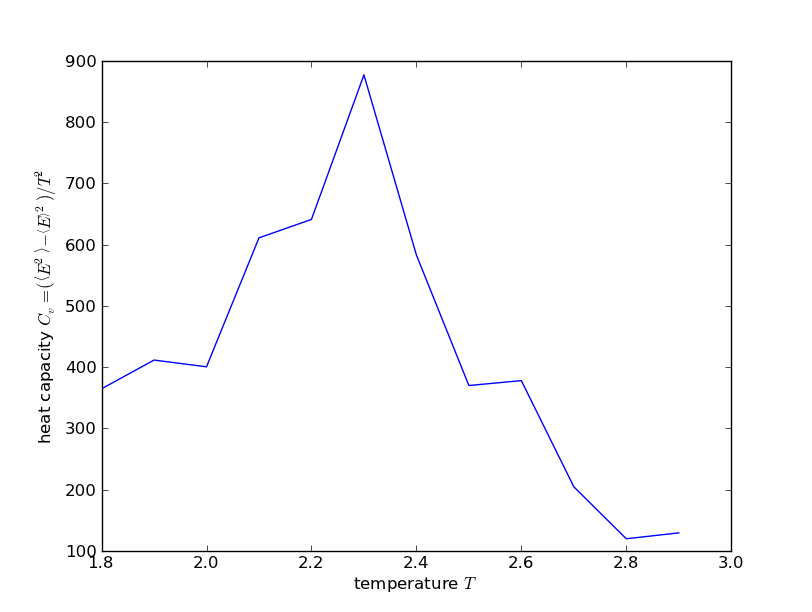
\includegraphics{cv.png}\hfill}


\section{Study folding pathway: 1) create standard deviation and mean energy plots for Barnase}
\label{tutorial:study-folding-pathway-1-create-standard-deviation-and-mean-energy-plots-for-barnase}
\begin{Verbatim}[commandchars=\\\{\}]
\PYG{c}{\PYGZsh{}!/usr/bin/env python}
\PYG{c}{\PYGZsh{} 2013, Michal Jamroz, public domain. http://biocomp.chem.uw.edu.pl}

\PYG{k+kn}{import} \PYG{n+nn}{os}\PYG{o}{,} \PYG{n+nn}{random}\PYG{o}{,} \PYG{n+nn}{pylab}\PYG{o}{,} \PYG{n+nn}{glob}\PYG{o}{,} \PYG{n+nn}{pycabs}\PYG{o}{,} \PYG{n+nn}{numpy} \PYG{k+kn}{as} \PYG{n+nn}{np}\PYG{o}{,} \PYG{n+nn}{multiprocessing} \PYG{k+kn}{as} \PYG{n+nn}{mp}
\PYG{c}{\PYGZsh{} first of all, download pyCABS and set self.FF = "" to the FF directory with cabs files}
\PYG{c}{\PYGZsh{} to compile CABS, use: g77 -O2 -ffloat-store -static -o cabs CABS.f }
\PYG{c}{\PYGZsh{} to compile CABS\PYGZus{}dynamics, use: g77 -O2 -ffloat-store -static -o cabs\PYGZus{}dynamics CABS\PYGZus{}dynamics.f }
\PYG{c}{\PYGZsh{} to compile lattice model builder, use g77 -O2 -ffloat-store -static build\PYGZus{}cabs61.f}
\PYG{c}{\PYGZsh{} in FF directory.}

\PYG{n}{sequence}\PYG{p}{,} \PYG{n}{secstr} \PYG{o}{=} \PYG{n}{pycabs}\PYG{o}{.}\PYG{n}{parseDSSPOutput}\PYG{p}{(}\PYG{l+s}{"}\PYG{l+s}{/where/is/my/barnase/1bnr.dssp}\PYG{l+s}{"}\PYG{p}{)} \PYG{c}{\PYGZsh{} define file with secondary structure definition of define sequence and secondary structure in sequence,secstr variables respectively}
\PYG{n}{name} \PYG{o}{=} \PYG{l+s}{"}\PYG{l+s}{barnase}\PYG{l+s}{"} \PYG{c}{\PYGZsh{} name for the project. Script will create subdirectories with this name as suffix}
\PYG{n}{template} \PYG{o}{=} \PYG{p}{[}\PYG{l+s}{"}\PYG{l+s}{/where/is/my/barnase/1bnr.pdb}\PYG{l+s}{"}\PYG{p}{]} \PYG{c}{\PYGZsh{} set path to the start structure (here - native structure). If user want to start from random chain, set template=[]. Note that path is relative to simulation directory}
\PYG{n}{independent\PYGZus{}runs}\PYG{o}{=}\PYG{l+m+mi}{5}  \PYG{c}{\PYGZsh{} set number of independent simulations for each temperature}
\PYG{n}{temp\PYGZus{}from} \PYG{o}{=} \PYG{l+m+mf}{1.5}     \PYG{c}{\PYGZsh{} define range of simulation temperatures, here is 1.0 - 2.8 with interval of 0.1}
\PYG{n}{temp\PYGZus{}to}  \PYG{o}{=} \PYG{l+m+mf}{3.8}
\PYG{n}{temp\PYGZus{}interval} \PYG{o}{=} \PYG{l+m+mf}{0.05}
\PYG{n}{temperatures}\PYG{o}{=}\PYG{n}{np}\PYG{o}{.}\PYG{n}{arange}\PYG{p}{(}\PYG{n}{temp\PYGZus{}from}\PYG{p}{,}\PYG{n}{temp\PYGZus{}to}\PYG{p}{,}\PYG{n}{temp\PYGZus{}interval}\PYG{p}{)}

\PYG{k}{def} \PYG{n+nf}{runCABS}\PYG{p}{(}\PYG{n}{temperature}\PYG{p}{)}\PYG{p}{:}
   \PYG{k}{global} \PYG{n}{name}\PYG{p}{,} \PYG{n}{sequence}\PYG{p}{,}\PYG{n}{secstr}\PYG{p}{,}\PYG{n}{template}\PYG{p}{,}\PYG{n}{independent\PYGZus{}runs}
   \PYG{n}{here} \PYG{o}{=} \PYG{n}{os}\PYG{o}{.}\PYG{n}{getcwd}\PYG{p}{(}\PYG{p}{)}
   \PYG{k}{for} \PYG{n}{i} \PYG{o+ow}{in} \PYG{n+nb}{range}\PYG{p}{(}\PYG{n}{independent\PYGZus{}runs}\PYG{p}{)}\PYG{p}{:}
      \PYG{n}{temp} \PYG{o}{=} \PYG{l+s}{"}\PYG{l+s+si}{\PYGZpc{}06.3f}\PYG{l+s}{"} \PYG{o}{\PYGZpc{}}\PYG{p}{(}\PYG{n}{temperature}\PYG{p}{)}
      \PYG{n}{dir\PYGZus{}name}\PYG{o}{=} \PYG{n}{name}\PYG{o}{+}\PYG{l+s}{"}\PYG{l+s}{\PYGZus{}}\PYG{l+s}{"}\PYG{o}{+}\PYG{n+nb}{str}\PYG{p}{(}\PYG{n}{i}\PYG{p}{)}\PYG{o}{+}\PYG{l+s}{"}\PYG{l+s}{\PYGZus{}T}\PYG{l+s}{"}\PYG{o}{+}\PYG{n}{temp}  \PYG{c}{\PYGZsh{} create unique name for simulation dir}
      \PYG{n}{a} \PYG{o}{=} \PYG{n}{pycabs}\PYG{o}{.}\PYG{n}{CABS}\PYG{p}{(}\PYG{n}{sequence}\PYG{p}{,}\PYG{n}{secstr}\PYG{p}{,}\PYG{n}{template}\PYG{p}{,}\PYG{n}{dir\PYGZus{}name}\PYG{p}{)} 
      \PYG{n}{a}\PYG{o}{.}\PYG{n}{rng\PYGZus{}seed} \PYG{o}{=} \PYG{n}{random}\PYG{o}{.}\PYG{n}{randint}\PYG{p}{(}\PYG{l+m+mi}{1}\PYG{p}{,}\PYG{l+m+mi}{10000}\PYG{p}{)} \PYG{c}{\PYGZsh{} set random generator seed for each independent simulation}
      \PYG{n}{a}\PYG{o}{.}\PYG{n}{createLatticeReplicas}\PYG{p}{(}\PYG{n}{replicas}\PYG{o}{=}\PYG{l+m+mi}{1}\PYG{p}{)}  \PYG{c}{\PYGZsh{} create lattice model for CABS}
      \PYG{n}{a}\PYG{o}{.}\PYG{n}{modeling}\PYG{p}{(}\PYG{n}{Ltemp}\PYG{o}{=}\PYG{n}{temperature}\PYG{p}{,}\PYG{n}{Htemp}\PYG{o}{=}\PYG{n}{temperature}\PYG{p}{,} \PYG{n}{phot}\PYG{o}{=}\PYG{l+m+mi}{300}\PYG{p}{,}\PYG{n}{cycles}\PYG{o}{=}\PYG{l+m+mi}{100}\PYG{p}{,}\PYG{n}{dynamics}\PYG{o}{=}\PYG{n+nb+bp}{True}\PYG{p}{)} \PYG{c}{\PYGZsh{} start modeling. phot is CABS microcycle, cycles variable is CABS macrocycle (how often write to the trajectory file)}
      \PYG{n}{os}\PYG{o}{.}\PYG{n}{chdir}\PYG{p}{(}\PYG{n}{here}\PYG{p}{)}

\PYG{n}{pool} \PYG{o}{=} \PYG{n}{mp}\PYG{o}{.}\PYG{n}{Pool}\PYG{p}{(}\PYG{p}{)}  \PYG{c}{\PYGZsh{} it use all available CPUs on workstation. If user want to use only - for example two - CPUs, set pool = mp.Pool(2)}
\PYG{n}{pool}\PYG{o}{.}\PYG{n}{map}\PYG{p}{(}\PYG{n}{runCABS}\PYG{p}{,}\PYG{n}{temperatures}\PYG{p}{)} \PYG{c}{\PYGZsh{} run simulations in parallel way, each simulation on each available CPU}

\PYG{c}{\PYGZsh{} postprocessing (comment out two lines above to avoid starting over simulations. If you want to only plot with other labels, etc. )}

\PYG{n}{cv} \PYG{o}{=} \PYG{n}{np}\PYG{o}{.}\PYG{n}{empty}\PYG{p}{(}\PYG{p}{[}\PYG{n}{independent\PYGZus{}runs}\PYG{p}{,}\PYG{n+nb}{len}\PYG{p}{(}\PYG{n}{temperatures}\PYG{p}{)}\PYG{p}{]}\PYG{p}{)}
\PYG{n}{avgene} \PYG{o}{=} \PYG{n}{np}\PYG{o}{.}\PYG{n}{empty}\PYG{p}{(}\PYG{p}{[}\PYG{n}{independent\PYGZus{}runs}\PYG{p}{,}\PYG{n+nb}{len}\PYG{p}{(}\PYG{n}{temperatures}\PYG{p}{)}\PYG{p}{]}\PYG{p}{)}
\PYG{k}{for} \PYG{n}{j} \PYG{o+ow}{in} \PYG{n+nb}{range}\PYG{p}{(}\PYG{n}{independent\PYGZus{}runs}\PYG{p}{)}\PYG{p}{:}
   \PYG{k}{for} \PYG{n}{i} \PYG{o+ow}{in} \PYG{n+nb}{range}\PYG{p}{(}\PYG{n+nb}{len}\PYG{p}{(}\PYG{n}{temperatures}\PYG{p}{)}\PYG{p}{)}\PYG{p}{:}
      \PYG{n}{t} \PYG{o}{=} \PYG{n}{temperatures}\PYG{p}{[}\PYG{n}{i}\PYG{p}{]}
      \PYG{n}{temp} \PYG{o}{=} \PYG{l+s}{"}\PYG{l+s+si}{\PYGZpc{}06.3f}\PYG{l+s}{"} \PYG{o}{\PYGZpc{}}\PYG{p}{(}\PYG{n}{t}\PYG{p}{)}
      \PYG{n}{e\PYGZus{}path} \PYG{o}{=} \PYG{n}{os}\PYG{o}{.}\PYG{n}{path}\PYG{o}{.}\PYG{n}{join}\PYG{p}{(}\PYG{n}{name}\PYG{o}{+}\PYG{l+s}{'}\PYG{l+s}{\PYGZus{}}\PYG{l+s}{'}\PYG{o}{+}\PYG{n+nb}{str}\PYG{p}{(}\PYG{n}{j}\PYG{p}{)}\PYG{o}{+}\PYG{l+s}{'}\PYG{l+s}{\PYGZus{}T}\PYG{l+s}{'}\PYG{o}{+}\PYG{n}{temp}\PYG{p}{,}\PYG{l+s}{'}\PYG{l+s}{ENERGY}\PYG{l+s}{'}\PYG{p}{)} \PYG{c}{\PYGZsh{} path constructed in the same way like dir\PYGZus{}name in runCABS definition above}
      \PYG{n}{energy} \PYG{o}{=} \PYG{n}{np}\PYG{o}{.}\PYG{n}{fromfile}\PYG{p}{(}\PYG{n}{e\PYGZus{}path}\PYG{p}{,}\PYG{n}{sep}\PYG{o}{=}\PYG{l+s}{'}\PYG{l+s+se}{\PYGZbs{}n}\PYG{l+s}{'}\PYG{p}{)}\PYG{p}{[}\PYG{l+m+mi}{1000}\PYG{p}{:}\PYG{p}{]} \PYG{c}{\PYGZsh{} read CABS energies for each trajectory model (second half)}
      \PYG{n}{cv}\PYG{p}{[}\PYG{n}{j}\PYG{p}{]}\PYG{p}{[}\PYG{n}{i}\PYG{p}{]} \PYG{o}{=} \PYG{n}{np}\PYG{o}{.}\PYG{n}{std}\PYG{p}{(}\PYG{n}{energy}\PYG{p}{)}  \PYG{c}{\PYGZsh{} calculate standard deviation (numpy std function) of energy, for each independent simulation}
      \PYG{n}{avgene}\PYG{p}{[}\PYG{n}{j}\PYG{p}{]}\PYG{p}{[}\PYG{n}{i}\PYG{p}{]} \PYG{o}{=} \PYG{n}{np}\PYG{o}{.}\PYG{n}{mean}\PYG{p}{(}\PYG{n}{energy}\PYG{p}{)} \PYG{c}{\PYGZsh{} calculate mean (numpy mean function) of energy}


\PYG{n}{mean\PYGZus{}sigma} \PYG{o}{=} \PYG{n}{np}\PYG{o}{.}\PYG{n}{mean}\PYG{p}{(}\PYG{n}{cv}\PYG{p}{,}\PYG{n}{axis}\PYG{o}{=}\PYG{l+m+mi}{0}\PYG{p}{)}    \PYG{c}{\PYGZsh{} average over independent simulations}
\PYG{n}{stddev\PYGZus{}sigma} \PYG{o}{=} \PYG{n}{np}\PYG{o}{.}\PYG{n}{std}\PYG{p}{(}\PYG{n}{cv}\PYG{p}{,}\PYG{n}{axis}\PYG{o}{=}\PYG{l+m+mi}{0}\PYG{p}{)}
\PYG{n}{mean\PYGZus{}ene} \PYG{o}{=} \PYG{n}{np}\PYG{o}{.}\PYG{n}{mean}\PYG{p}{(}\PYG{n}{avgene}\PYG{p}{,}\PYG{n}{axis}\PYG{o}{=}\PYG{l+m+mi}{0}\PYG{p}{)}  \PYG{c}{\PYGZsh{} calculate of standard deviations and mean values over independent simulations}
\PYG{n}{stddev\PYGZus{}ene} \PYG{o}{=} \PYG{n}{np}\PYG{o}{.}\PYG{n}{std}\PYG{p}{(}\PYG{n}{avgene}\PYG{p}{,}\PYG{n}{axis}\PYG{o}{=}\PYG{l+m+mi}{0}\PYG{p}{)}

\PYG{c}{\PYGZsh{} plotting data with pylab python module. Read matplotlib manual (http://matplotlib.org/) for explanation of below code}
\PYG{n}{pylab}\PYG{o}{.}\PYG{n}{ylabel}\PYG{p}{(}\PYG{l+s}{r'}\PYG{l+s}{Standard deviation of energy}\PYG{l+s}{'} \PYG{p}{)}
\PYG{n}{pylab}\PYG{o}{.}\PYG{n}{xlabel}\PYG{p}{(}\PYG{l+s}{r'}\PYG{l+s}{Temperature, \PYGZdl{}T\PYGZdl{}}\PYG{l+s}{'}\PYG{p}{)}
\PYG{n}{pylab}\PYG{o}{.}\PYG{n}{xlim}\PYG{p}{(}\PYG{n}{temp\PYGZus{}from}\PYG{p}{,}\PYG{n}{temp\PYGZus{}to}\PYG{p}{)}
\PYG{k}{for} \PYG{n}{i} \PYG{o+ow}{in} \PYG{n+nb}{range}\PYG{p}{(}\PYG{n}{independent\PYGZus{}runs}\PYG{p}{)}\PYG{p}{:}
    \PYG{n}{pylab}\PYG{o}{.}\PYG{n}{plot}\PYG{p}{(}\PYG{n}{temperatures}\PYG{p}{,} \PYG{n}{cv}\PYG{p}{[}\PYG{n}{i}\PYG{p}{]}\PYG{p}{,} \PYG{l+s}{'}\PYG{l+s}{.}\PYG{l+s}{'}\PYG{p}{)}
\PYG{n}{pylab}\PYG{o}{.}\PYG{n}{errorbar}\PYG{p}{(}\PYG{n}{temperatures}\PYG{p}{,}\PYG{n}{mean\PYGZus{}sigma}\PYG{p}{,}\PYG{n}{yerr}\PYG{o}{=}\PYG{n}{stddev\PYGZus{}sigma}\PYG{p}{,}\PYG{n}{fmt}\PYG{o}{=}\PYG{l+s}{'}\PYG{l+s}{o-}\PYG{l+s}{'}\PYG{p}{)}
\PYG{n}{pylab}\PYG{o}{.}\PYG{n}{savefig}\PYG{p}{(}\PYG{l+s}{"}\PYG{l+s}{stdE\PYGZus{}barnase.png}\PYG{l+s}{"}\PYG{p}{,}\PYG{n}{dpi}\PYG{o}{=}\PYG{l+m+mi}{600}\PYG{p}{)}
\PYG{n}{pylab}\PYG{o}{.}\PYG{n}{close}\PYG{p}{(}\PYG{p}{)}

\PYG{n}{pylab}\PYG{o}{.}\PYG{n}{ylabel}\PYG{p}{(}\PYG{l+s}{r'}\PYG{l+s}{Mean energy}\PYG{l+s}{'} \PYG{p}{)}
\PYG{n}{pylab}\PYG{o}{.}\PYG{n}{xlabel}\PYG{p}{(}\PYG{l+s}{r'}\PYG{l+s}{Temperature, \PYGZdl{}T\PYGZdl{}}\PYG{l+s}{'}\PYG{p}{)}
\PYG{n}{pylab}\PYG{o}{.}\PYG{n}{xlim}\PYG{p}{(}\PYG{n}{temp\PYGZus{}from}\PYG{p}{,}\PYG{n}{temp\PYGZus{}to}\PYG{p}{)}
\PYG{k}{for} \PYG{n}{i} \PYG{o+ow}{in} \PYG{n+nb}{range}\PYG{p}{(}\PYG{n}{independent\PYGZus{}runs}\PYG{p}{)}\PYG{p}{:}
    \PYG{n}{pylab}\PYG{o}{.}\PYG{n}{plot}\PYG{p}{(}\PYG{n}{temperatures}\PYG{p}{,} \PYG{n}{avgene}\PYG{p}{[}\PYG{n}{i}\PYG{p}{]}\PYG{p}{,} \PYG{l+s}{'}\PYG{l+s}{.}\PYG{l+s}{'}\PYG{p}{)}
\PYG{n}{pylab}\PYG{o}{.}\PYG{n}{errorbar}\PYG{p}{(}\PYG{n}{temperatures}\PYG{p}{,}\PYG{n}{mean\PYGZus{}ene}\PYG{p}{,}\PYG{n}{yerr}\PYG{o}{=}\PYG{n}{stddev\PYGZus{}ene}\PYG{p}{,}\PYG{n}{fmt}\PYG{o}{=}\PYG{l+s}{'}\PYG{l+s}{o-}\PYG{l+s}{'}\PYG{p}{)}
\PYG{n}{pylab}\PYG{o}{.}\PYG{n}{savefig}\PYG{p}{(}\PYG{l+s}{"}\PYG{l+s}{meanE\PYGZus{}barnase.png}\PYG{l+s}{"}\PYG{p}{,}\PYG{n}{dpi}\PYG{o}{=}\PYG{l+m+mi}{600}\PYG{p}{)}
\PYG{n}{pylab}\PYG{o}{.}\PYG{n}{close}\PYG{p}{(}\PYG{p}{)}


\PYG{c}{\PYGZsh{} as a results user will get a lot of barnase* subdirectories, stdE\PYGZus{}barnase.png and meanE\PYGZus{}barnase.png files.}
\PYG{c}{\PYGZsh{} EOF}
\end{Verbatim}

Download script: \code{folding\_pathway.py}.
Download necessary files: \code{1bnr.pdb}, \code{1bnr.dssp}

Results:

{\hfill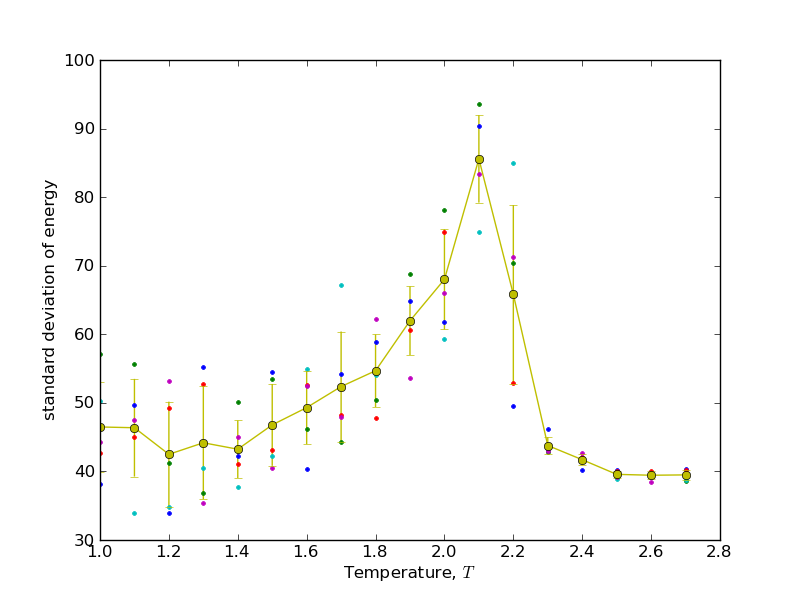
\includegraphics{stdE_barnase.png}\hfill}

{\hfill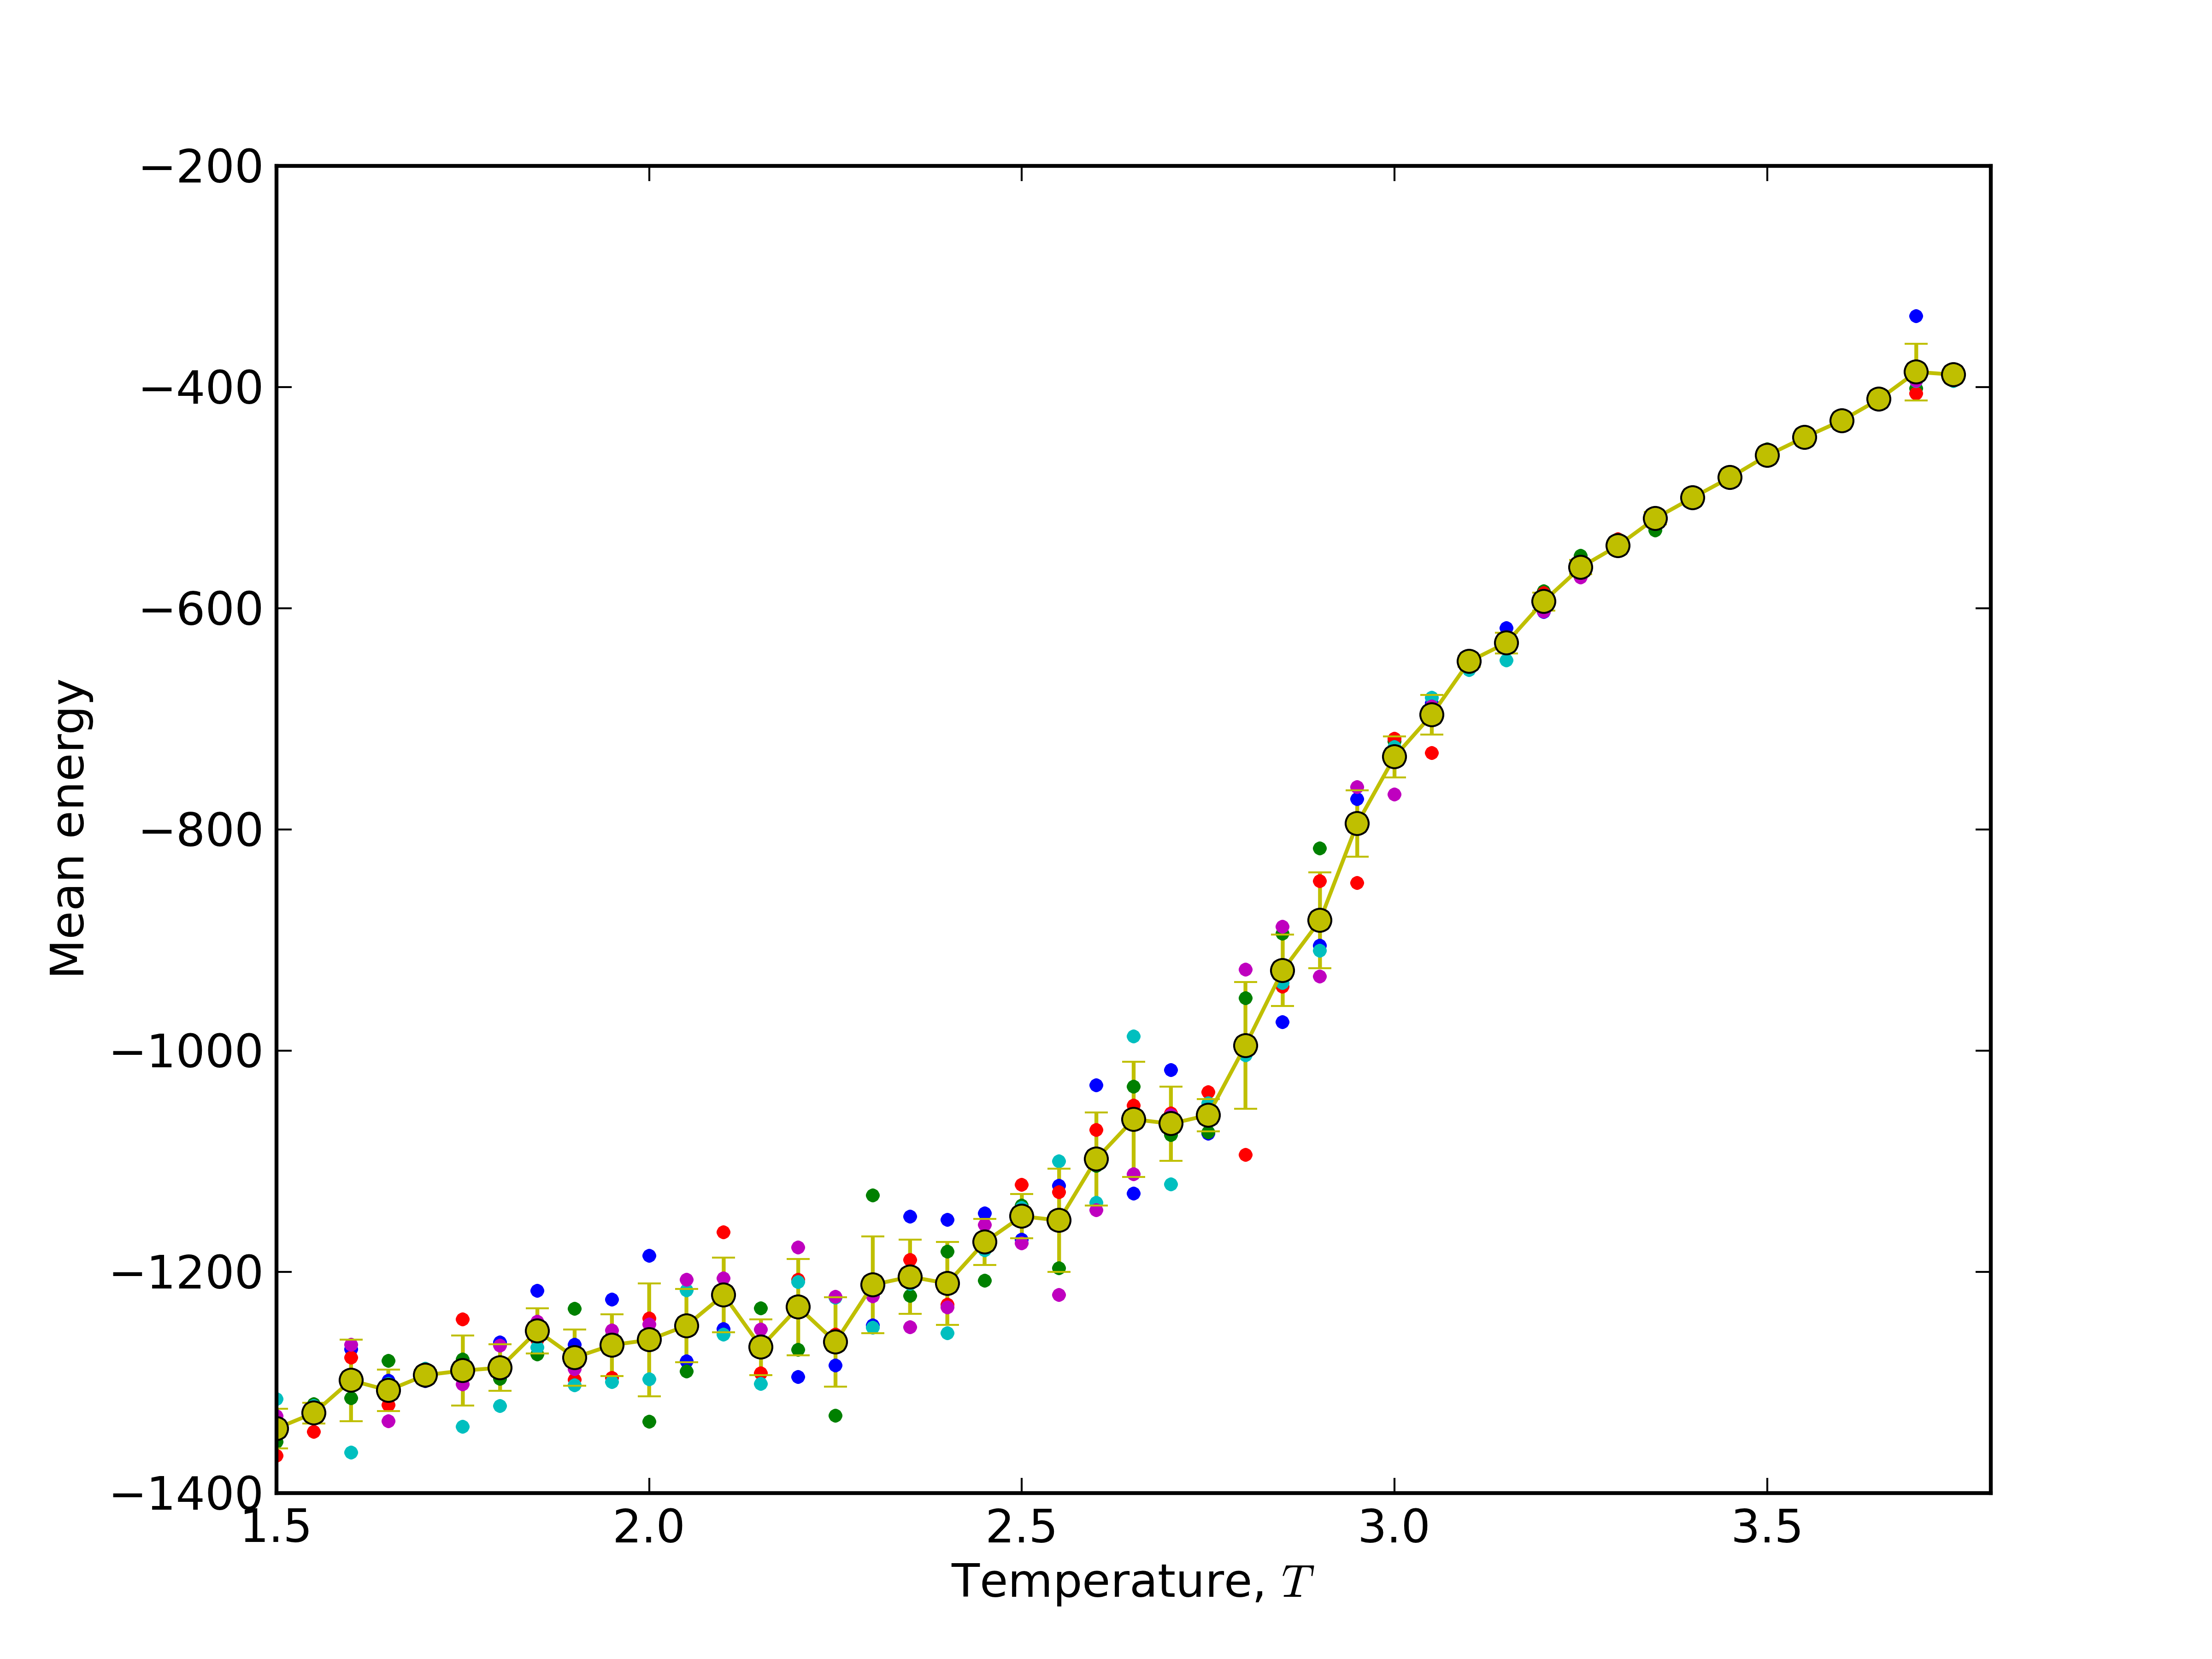
\includegraphics{meanE_barnase.png}\hfill}


\section{Study folding pathway: 2) calculate average contact map over trajectory of sidegroups in temperature 2.1}
\label{tutorial:study-folding-pathway-2-calculate-average-contact-map-over-trajectory-of-sidegroups-in-temperature-2-1}
\begin{Verbatim}[commandchars=\\\{\}]
\PYG{c}{\PYGZsh{}!/usr/bin/env python}
\PYG{c}{\PYGZsh{} 2013, Michal Jamroz, public domain. http://biocomp.chem.uw.edu.pl}
\PYG{k+kn}{import} \PYG{n+nn}{pycabs}\PYG{o}{,}\PYG{n+nn}{os}\PYG{o}{,}\PYG{n+nn}{numpy} \PYG{k+kn}{as} \PYG{n+nn}{np}

\PYG{n}{name} \PYG{o}{=} \PYG{l+s}{"}\PYG{l+s}{barnase}\PYG{l+s}{"} \PYG{c}{\PYGZsh{} set project name same like in folding\PYGZus{}pathway.py script}
\PYG{n}{max\PYGZus{}sd\PYGZus{}temperature}\PYG{o}{=}\PYG{l+m+mf}{2.9} \PYG{c}{\PYGZsh{} read from the plot temperature for which maximum deviation of energy is observed}
\PYG{n}{independent\PYGZus{}runs}\PYG{o}{=}\PYG{l+m+mi}{5}     \PYG{c}{\PYGZsh{} set the same value like in folding\PYGZus{}pathway.py script}

\PYG{c}{\PYGZsh{} read trajectory of sidegroups (TRASG) from all independent simulations to the trajectory variable}
\PYG{n}{trajectory} \PYG{o}{=} \PYG{p}{[}\PYG{p}{]}
\PYG{k}{for} \PYG{n}{j} \PYG{o+ow}{in} \PYG{n+nb}{range}\PYG{p}{(}\PYG{n}{independent\PYGZus{}runs}\PYG{p}{)}\PYG{p}{:}
	\PYG{n}{temp} \PYG{o}{=} \PYG{l+s}{"}\PYG{l+s+si}{\PYGZpc{}06.3f}\PYG{l+s}{"} \PYG{o}{\PYGZpc{}}\PYG{p}{(}\PYG{n}{max\PYGZus{}sd\PYGZus{}temperature}\PYG{p}{)}
	\PYG{n}{e\PYGZus{}path} \PYG{o}{=} \PYG{n}{os}\PYG{o}{.}\PYG{n}{path}\PYG{o}{.}\PYG{n}{join}\PYG{p}{(}\PYG{n}{name}\PYG{o}{+}\PYG{l+s}{'}\PYG{l+s}{\PYGZus{}}\PYG{l+s}{'}\PYG{o}{+}\PYG{n+nb}{str}\PYG{p}{(}\PYG{n}{j}\PYG{p}{)}\PYG{o}{+}\PYG{l+s}{'}\PYG{l+s}{\PYGZus{}T}\PYG{l+s}{'}\PYG{o}{+}\PYG{n}{temp}\PYG{p}{,}\PYG{l+s}{'}\PYG{l+s}{TRASG}\PYG{l+s}{'}\PYG{p}{)}
	\PYG{n}{trajectory} \PYG{o}{+}\PYG{o}{=} \PYG{n}{pycabs}\PYG{o}{.}\PYG{n}{loadSGCoordinates}\PYG{p}{(}\PYG{n}{e\PYGZus{}path}\PYG{p}{)}\PYG{p}{[}\PYG{l+m+mi}{1000}\PYG{p}{:}\PYG{p}{]} \PYG{c}{\PYGZsh{} second half of sidechains trajectory}

\PYG{n}{contact} \PYG{o}{=} \PYG{n}{pycabs}\PYG{o}{.}\PYG{n}{contact\PYGZus{}map}\PYG{p}{(}\PYG{n}{trajectory}\PYG{p}{,}\PYG{l+m+mf}{7.0}\PYG{p}{)} \PYG{c}{\PYGZsh{} calculate averaged contact map over trajectories. Cutoff set to 7.0A.}

\PYG{c}{\PYGZsh{} plot contact map with pylab. Read matplotlib manual (http://matplotlib.org/) for explanation of the code below}
\PYG{k+kn}{from} \PYG{n+nn}{pylab} \PYG{k+kn}{import} \PYG{n}{xlabel}\PYG{p}{,}\PYG{n}{ylabel}\PYG{p}{,}\PYG{n}{pcolor}\PYG{p}{,}\PYG{n}{colorbar}\PYG{p}{,}\PYG{n}{savefig}\PYG{p}{,}\PYG{n}{xlim}\PYG{p}{,}\PYG{n}{ylim}\PYG{p}{,}\PYG{n}{cm}
\PYG{k+kn}{from} \PYG{n+nn}{numpy} \PYG{k+kn}{import} \PYG{n}{indices}
\PYG{n}{l}\PYG{o}{=}\PYG{n+nb}{len}\PYG{p}{(}\PYG{n}{trajectory}\PYG{p}{[}\PYG{l+m+mi}{0}\PYG{p}{]}\PYG{p}{)}
\PYG{n}{rows}\PYG{p}{,} \PYG{n}{cols} \PYG{o}{=} \PYG{n}{indices}\PYG{p}{(}\PYG{p}{(}\PYG{n}{l}\PYG{p}{,}\PYG{n}{l}\PYG{p}{)}\PYG{p}{)}
\PYG{n}{xlabel}\PYG{p}{(}\PYG{l+s}{"}\PYG{l+s}{Residue index}\PYG{l+s}{"}\PYG{p}{)}
\PYG{n}{xlim}\PYG{p}{(}\PYG{l+m+mi}{0}\PYG{p}{,} \PYG{n+nb}{len}\PYG{p}{(}\PYG{n}{contact}\PYG{p}{)}\PYG{p}{)}
\PYG{n}{ylim}\PYG{p}{(}\PYG{l+m+mi}{0}\PYG{p}{,} \PYG{n+nb}{len}\PYG{p}{(}\PYG{n}{contact}\PYG{p}{)}\PYG{p}{)}
\PYG{n}{ylabel}\PYG{p}{(}\PYG{l+s}{"}\PYG{l+s}{Residue index}\PYG{l+s}{"}\PYG{p}{)}
\PYG{n}{pcolor}\PYG{p}{(}\PYG{n}{contact}\PYG{p}{,} \PYG{n}{cmap}\PYG{o}{=}\PYG{n}{cm}\PYG{o}{.}\PYG{n}{gnuplot2\PYGZus{}r}\PYG{p}{,}\PYG{n}{vmax}\PYG{o}{=}\PYG{l+m+mf}{0.6}\PYG{p}{)} \PYG{c}{\PYGZsh{} vmax is range of colorbar. Here is set to 0.8, which gave white color for all values greater than 0.8}
\PYG{n}{cb} \PYG{o}{=} \PYG{n}{colorbar}\PYG{p}{(}\PYG{p}{)}
\PYG{n}{cb}\PYG{o}{.}\PYG{n}{set\PYGZus{}label}\PYG{p}{(}\PYG{l+s}{"}\PYG{l+s}{Fraction of contacts}\PYG{l+s}{"}\PYG{p}{)}
\PYG{n}{savefig}\PYG{p}{(}\PYG{l+s}{"}\PYG{l+s}{heatmap}\PYG{l+s}{"}\PYG{o}{+}\PYG{n+nb}{str}\PYG{p}{(}\PYG{n}{max\PYGZus{}sd\PYGZus{}temperature}\PYG{p}{)}\PYG{o}{+}\PYG{l+s}{"}\PYG{l+s}{.png}\PYG{l+s}{"}\PYG{p}{,}\PYG{n}{dpi}\PYG{o}{=}\PYG{l+m+mi}{600}\PYG{p}{)}

\PYG{c}{\PYGZsh{} optionally, write contact map values into the text file formatted for GNUplot}
\PYG{n}{fw} \PYG{o}{=} \PYG{n+nb}{open}\PYG{p}{(}\PYG{l+s}{"}\PYG{l+s}{contact\PYGZus{}map.dat}\PYG{l+s}{"}\PYG{p}{,}\PYG{l+s}{"}\PYG{l+s}{w}\PYG{l+s}{"}\PYG{p}{)}
\PYG{k}{for} \PYG{n}{i} \PYG{o+ow}{in} \PYG{n+nb}{range}\PYG{p}{(}\PYG{n+nb}{len}\PYG{p}{(}\PYG{n}{contact}\PYG{p}{)}\PYG{p}{)}\PYG{p}{:}
   \PYG{k}{for} \PYG{n}{j} \PYG{o+ow}{in} \PYG{n+nb}{range}\PYG{p}{(}\PYG{n+nb}{len}\PYG{p}{(}\PYG{n}{contact}\PYG{p}{)}\PYG{p}{)}\PYG{p}{:}
      \PYG{n}{fw}\PYG{o}{.}\PYG{n}{write}\PYG{p}{(}\PYG{l+s}{"}\PYG{l+s+si}{\PYGZpc{}5d}\PYG{l+s}{ }\PYG{l+s+si}{\PYGZpc{}5d}\PYG{l+s}{ }\PYG{l+s+si}{\PYGZpc{}7.5f}\PYG{l+s+se}{\PYGZbs{}n}\PYG{l+s}{"} \PYG{o}{\PYGZpc{}}\PYG{p}{(}\PYG{n}{i}\PYG{o}{+}\PYG{l+m+mi}{1}\PYG{p}{,}\PYG{n}{j}\PYG{o}{+}\PYG{l+m+mi}{1}\PYG{p}{,}\PYG{n}{contact}\PYG{p}{[}\PYG{n}{i}\PYG{p}{]}\PYG{p}{[}\PYG{n}{j}\PYG{p}{]}\PYG{p}{)}\PYG{p}{)}
   \PYG{n}{fw}\PYG{o}{.}\PYG{n}{write}\PYG{p}{(}\PYG{l+s}{"}\PYG{l+s+se}{\PYGZbs{}n}\PYG{l+s}{"}\PYG{p}{)}
\PYG{n}{fw}\PYG{o}{.}\PYG{n}{close}\PYG{p}{(}\PYG{p}{)}

\PYG{c}{\PYGZsh{} example GNUplot script for plotting contact map of contact\PYGZus{}map.dat file:}
\PYG{l+s+sd}{'''}
\PYG{l+s+sd}{set terminal unknown}
\PYG{l+s+sd}{plot 'contact\PYGZus{}map.dat' using 1:2:3}
\PYG{l+s+sd}{set xrange[GPVAL\PYGZus{}DATA\PYGZus{}X\PYGZus{}MIN:GPVAL\PYGZus{}DATA\PYGZus{}X\PYGZus{}MAX]}
\PYG{l+s+sd}{set yrange[GPVAL\PYGZus{}DATA\PYGZus{}Y\PYGZus{}MIN:GPVAL\PYGZus{}DATA\PYGZus{}Y\PYGZus{}MAX]}


\PYG{l+s+sd}{set terminal postscript eps enhanced color "Helvetica" 14}
\PYG{l+s+sd}{set output 'contact\PYGZus{}map.eps'}
\PYG{l+s+sd}{set size ratio 1}
\PYG{l+s+sd}{unset key}
\PYG{l+s+sd}{set xlabel 'Residue index'}
\PYG{l+s+sd}{set ylabel 'Residue index'}
\PYG{l+s+sd}{set cbrange[:0.8]}
\PYG{l+s+sd}{set palette negative}
\PYG{l+s+sd}{plot 'contact\PYGZus{}map.dat' with image}
\PYG{l+s+sd}{'''}

\PYG{c}{\PYGZsh{} write it to the file.gp and run: gnuplot file.gp to get postscript file with heat map plot}
\end{Verbatim}

Download script: \code{contact\_map.py}.

Results:

{\hfill\includegraphics{heatmap29.png}\hfill}

Optionally, GNUplot script for plotting contact\_map.dat file generated by contact\_map.py script:

\begin{Verbatim}[commandchars=\\\{\}]
set terminal unknown
plot 'contact\_map.dat' using 1:2:3
set xrange[GPVAL\_DATA\_X\_MIN:GPVAL\_DATA\_X\_MAX]
set yrange[GPVAL\_DATA\_Y\_MIN:GPVAL\_DATA\_Y\_MAX]


set terminal postscript eps enhanced color "Helvetica" 14
set output 'contact\_map.eps'
set size ratio 1
unset key
set xlabel 'Residue index'
set ylabel 'Residue index'
set cbrange[:0.8]
set palette negative
plot 'contact\_map.dat' with image
\end{Verbatim}

Download script: \code{gnuplot\_script.gp}.


\section{Monitoring of CABS energy during simulation}
\label{tutorial:monitoring-of-cabs-energy-during-simulation}
\begin{Verbatim}[commandchars=\\\{\}]
\PYG{c}{\PYGZsh{}!/usr/bin/env python}
\PYG{k+kn}{from} \PYG{n+nn}{pylab} \PYG{k+kn}{import} \PYG{o}{*}
\PYG{k+kn}{from} \PYG{n+nn}{sys} \PYG{k+kn}{import} \PYG{n}{argv}
\PYG{k+kn}{import} \PYG{n+nn}{os}
\PYG{k+kn}{import} \PYG{n+nn}{time}
\PYG{k+kn}{import} \PYG{n+nn}{numpy} \PYG{k+kn}{as} \PYG{n+nn}{np}
\PYG{k+kn}{import} \PYG{n+nn}{pycabs}

\PYG{k}{class} \PYG{n+nc}{Energy}\PYG{p}{(}\PYG{n}{pycabs}\PYG{o}{.}\PYG{n}{Calculate}\PYG{p}{)}\PYG{p}{:}
    \PYG{k}{def} \PYG{n+nf}{calculate}\PYG{p}{(}\PYG{n+nb+bp}{self}\PYG{p}{,}\PYG{n}{data}\PYG{p}{)}\PYG{p}{:}
        \PYG{k}{for} \PYG{n}{i} \PYG{o+ow}{in} \PYG{n}{data}\PYG{p}{:}
            \PYG{n+nb+bp}{self}\PYG{o}{.}\PYG{n}{out}\PYG{o}{.}\PYG{n}{append}\PYG{p}{(}\PYG{n+nb}{float}\PYG{p}{(}\PYG{n}{i}\PYG{p}{)}\PYG{p}{)} \PYG{c}{\PYGZsh{} ENERGY file contains one value in a row}
            
\PYG{n}{out} \PYG{o}{=} \PYG{p}{[}\PYG{p}{]}						
\PYG{n}{calc} \PYG{o}{=} \PYG{n}{Energy}\PYG{p}{(}\PYG{n}{out}\PYG{p}{)} \PYG{c}{\PYGZsh{} out is dynamically updated }
\PYG{n}{m}\PYG{o}{=}\PYG{n}{pycabs}\PYG{o}{.}\PYG{n}{Monitor}\PYG{p}{(}\PYG{n}{os}\PYG{o}{.}\PYG{n}{path}\PYG{o}{.}\PYG{n}{join}\PYG{p}{(}\PYG{n}{argv}\PYG{p}{[}\PYG{l+m+mi}{1}\PYG{p}{]}\PYG{p}{,}\PYG{l+s}{"}\PYG{l+s}{ENERGY}\PYG{l+s}{"}\PYG{p}{)}\PYG{p}{,}\PYG{n}{calc}\PYG{p}{)}
\PYG{n}{m}\PYG{o}{.}\PYG{n}{daemon} \PYG{o}{=} \PYG{n+nb+bp}{True}
\PYG{n}{m}\PYG{o}{.}\PYG{n}{start}\PYG{p}{(}\PYG{p}{)}



\PYG{n}{ion}\PYG{p}{(}\PYG{p}{)}
\PYG{n}{y} \PYG{o}{=} \PYG{n}{zeros}\PYG{p}{(}\PYG{l+m+mi}{1}\PYG{p}{)}
\PYG{n}{x} \PYG{o}{=} \PYG{n}{zeros}\PYG{p}{(}\PYG{l+m+mi}{1}\PYG{p}{)}
\PYG{n}{line}\PYG{p}{,} \PYG{o}{=} \PYG{n}{plot}\PYG{p}{(}\PYG{n}{x}\PYG{p}{,}\PYG{n}{y}\PYG{p}{)}
\PYG{n}{xlabel}\PYG{p}{(}\PYG{l+s}{'}\PYG{l+s}{CABS time step}\PYG{l+s}{'}\PYG{p}{)}
\PYG{n}{ylabel}\PYG{p}{(}\PYG{l+s}{'}\PYG{l+s}{CABS energy}\PYG{l+s}{'}\PYG{p}{)}

\PYG{k}{while} \PYG{l+m+mi}{1}\PYG{p}{:}
    \PYG{n}{time}\PYG{o}{.}\PYG{n}{sleep}\PYG{p}{(}\PYG{l+m+mi}{1}\PYG{p}{)}
    \PYG{n}{y} \PYG{o}{=} \PYG{n}{np}\PYG{o}{.}\PYG{n}{asarray}\PYG{p}{(}\PYG{n}{out}\PYG{p}{)}
    \PYG{n}{x} \PYG{o}{=} \PYG{n+nb}{xrange}\PYG{p}{(}\PYG{l+m+mi}{0}\PYG{p}{,}\PYG{n+nb}{len}\PYG{p}{(}\PYG{n}{out}\PYG{p}{)}\PYG{p}{)}
    \PYG{n}{axis}\PYG{p}{(}\PYG{p}{[}\PYG{l+m+mi}{0}\PYG{p}{,} \PYG{n}{amax}\PYG{p}{(}\PYG{n}{x}\PYG{p}{)}\PYG{o}{+}\PYG{l+m+mi}{1}\PYG{p}{,} \PYG{n}{amin}\PYG{p}{(}\PYG{n}{y}\PYG{p}{)}\PYG{o}{-}\PYG{l+m+mi}{5}\PYG{p}{,} \PYG{n}{amax}\PYG{p}{(}\PYG{n}{y}\PYG{p}{)}\PYG{o}{+}\PYG{l+m+mi}{5} \PYG{p}{]}\PYG{p}{)}
    \PYG{n}{line}\PYG{o}{.}\PYG{n}{set\PYGZus{}ydata}\PYG{p}{(}\PYG{n}{y}\PYG{p}{)}  \PYG{c}{\PYGZsh{} update the data}
    \PYG{n}{line}\PYG{o}{.}\PYG{n}{set\PYGZus{}xdata}\PYG{p}{(}\PYG{n}{x}\PYG{p}{)}
    \PYG{n}{draw}\PYG{p}{(}\PYG{p}{)}
\end{Verbatim}

Download script: \code{monitoring\_energy.py}.


\section{Monitoring of end-to-end distance of chain during simulation}
\label{tutorial:monitoring-of-end-to-end-distance-of-chain-during-simulation}
\begin{Verbatim}[commandchars=\\\{\}]
\PYG{c}{\PYGZsh{}!/usr/bin/env python}
\PYG{k+kn}{from} \PYG{n+nn}{pylab} \PYG{k+kn}{import} \PYG{o}{*}
\PYG{k+kn}{from} \PYG{n+nn}{sys} \PYG{k+kn}{import} \PYG{n}{argv}
\PYG{k+kn}{import} \PYG{n+nn}{time}
\PYG{k+kn}{import} \PYG{n+nn}{os}
\PYG{k+kn}{import} \PYG{n+nn}{numpy} \PYG{k+kn}{as} \PYG{n+nn}{np}
\PYG{k+kn}{import} \PYG{n+nn}{pycabs}

\PYG{k}{class} \PYG{n+nc}{E2E}\PYG{p}{(}\PYG{n}{pycabs}\PYG{o}{.}\PYG{n}{Calculate}\PYG{p}{)}\PYG{p}{:}
    \PYG{k}{def} \PYG{n+nf}{calculate}\PYG{p}{(}\PYG{n+nb+bp}{self}\PYG{p}{,}\PYG{n}{data}\PYG{p}{)}\PYG{p}{:}
        \PYG{n}{models} \PYG{o}{=} \PYG{n+nb+bp}{self}\PYG{o}{.}\PYG{n}{processTrajectory}\PYG{p}{(}\PYG{n}{data}\PYG{p}{)}
        \PYG{k}{for} \PYG{n}{m} \PYG{o+ow}{in} \PYG{n}{models}\PYG{p}{:}
            \PYG{n}{first} \PYG{o}{=} \PYG{n}{m}\PYG{p}{[}\PYG{l+m+mi}{0}\PYG{p}{:}\PYG{l+m+mi}{3}\PYG{p}{]}
            \PYG{n}{last} \PYG{o}{=} \PYG{n}{m}\PYG{p}{[}\PYG{o}{-}\PYG{l+m+mi}{3}\PYG{p}{:}\PYG{p}{]}

            \PYG{n}{x} \PYG{o}{=} \PYG{n}{first}\PYG{p}{[}\PYG{l+m+mi}{0}\PYG{p}{]}\PYG{o}{-}\PYG{n}{last}\PYG{p}{[}\PYG{l+m+mi}{0}\PYG{p}{]}
            \PYG{n}{y} \PYG{o}{=} \PYG{n}{first}\PYG{p}{[}\PYG{l+m+mi}{1}\PYG{p}{]}\PYG{o}{-}\PYG{n}{last}\PYG{p}{[}\PYG{l+m+mi}{1}\PYG{p}{]}
            \PYG{n}{z} \PYG{o}{=} \PYG{n}{first}\PYG{p}{[}\PYG{l+m+mi}{2}\PYG{p}{]}\PYG{o}{-}\PYG{n}{last}\PYG{p}{[}\PYG{l+m+mi}{2}\PYG{p}{]}
            \PYG{n+nb+bp}{self}\PYG{o}{.}\PYG{n}{out}\PYG{o}{.}\PYG{n}{append}\PYG{p}{(}\PYG{n}{x}\PYG{o}{*}\PYG{n}{x}\PYG{o}{+}\PYG{n}{y}\PYG{o}{*}\PYG{n}{y}\PYG{o}{+}\PYG{n}{z}\PYG{o}{*}\PYG{n}{z}\PYG{p}{)}            
            
\PYG{n}{out} \PYG{o}{=} \PYG{p}{[}\PYG{p}{]}						
\PYG{n}{calc} \PYG{o}{=} \PYG{n}{E2E}\PYG{p}{(}\PYG{n}{out}\PYG{p}{)} \PYG{c}{\PYGZsh{} out is dynamically updated }
\PYG{n}{m}\PYG{o}{=}\PYG{n}{pycabs}\PYG{o}{.}\PYG{n}{Monitor}\PYG{p}{(}\PYG{n}{os}\PYG{o}{.}\PYG{n}{path}\PYG{o}{.}\PYG{n}{join}\PYG{p}{(}\PYG{n}{argv}\PYG{p}{[}\PYG{l+m+mi}{1}\PYG{p}{]}\PYG{p}{,}\PYG{l+s}{"}\PYG{l+s}{TRAF}\PYG{l+s}{"}\PYG{p}{)}\PYG{p}{,}\PYG{n}{calc}\PYG{p}{)}
\PYG{n}{m}\PYG{o}{.}\PYG{n}{daemon} \PYG{o}{=} \PYG{n+nb+bp}{True}
\PYG{n}{m}\PYG{o}{.}\PYG{n}{start}\PYG{p}{(}\PYG{p}{)}


\PYG{n}{ion}\PYG{p}{(}\PYG{p}{)}
\PYG{n}{y} \PYG{o}{=} \PYG{n}{zeros}\PYG{p}{(}\PYG{l+m+mi}{1}\PYG{p}{)}
\PYG{n}{x} \PYG{o}{=} \PYG{n}{zeros}\PYG{p}{(}\PYG{l+m+mi}{1}\PYG{p}{)}
\PYG{n}{line}\PYG{p}{,} \PYG{o}{=} \PYG{n}{plot}\PYG{p}{(}\PYG{n}{x}\PYG{p}{,}\PYG{n}{y}\PYG{p}{)}
\PYG{n}{xlabel}\PYG{p}{(}\PYG{l+s}{'}\PYG{l+s}{CABS time step}\PYG{l+s}{'}\PYG{p}{)}
\PYG{n}{ylabel}\PYG{p}{(}\PYG{l+s}{'}\PYG{l+s}{square of end to end distance}\PYG{l+s}{'}\PYG{p}{)}

\PYG{k}{while} \PYG{l+m+mi}{1}\PYG{p}{:}
    \PYG{n}{time}\PYG{o}{.}\PYG{n}{sleep}\PYG{p}{(}\PYG{l+m+mi}{1}\PYG{p}{)}
    \PYG{n}{y} \PYG{o}{=} \PYG{n}{np}\PYG{o}{.}\PYG{n}{asarray}\PYG{p}{(}\PYG{n}{out}\PYG{p}{)}
    \PYG{n}{x} \PYG{o}{=} \PYG{n+nb}{xrange}\PYG{p}{(}\PYG{l+m+mi}{0}\PYG{p}{,}\PYG{n+nb}{len}\PYG{p}{(}\PYG{n}{out}\PYG{p}{)}\PYG{p}{)}
    \PYG{n}{axis}\PYG{p}{(}\PYG{p}{[}\PYG{l+m+mi}{0}\PYG{p}{,} \PYG{n}{amax}\PYG{p}{(}\PYG{n}{x}\PYG{p}{)}\PYG{o}{+}\PYG{l+m+mi}{1}\PYG{p}{,} \PYG{n}{amin}\PYG{p}{(}\PYG{n}{y}\PYG{p}{)}\PYG{o}{-}\PYG{l+m+mi}{5}\PYG{p}{,} \PYG{n}{amax}\PYG{p}{(}\PYG{n}{y}\PYG{p}{)}\PYG{o}{+}\PYG{l+m+mi}{5} \PYG{p}{]}\PYG{p}{)}
    \PYG{n}{line}\PYG{o}{.}\PYG{n}{set\PYGZus{}ydata}\PYG{p}{(}\PYG{n}{y}\PYG{p}{)}  \PYG{c}{\PYGZsh{} update the data}
    \PYG{n}{line}\PYG{o}{.}\PYG{n}{set\PYGZus{}xdata}\PYG{p}{(}\PYG{n}{x}\PYG{p}{)}
    \PYG{n}{draw}\PYG{p}{(}\PYG{p}{)}
\end{Verbatim}

Download script: \code{monitoring\_e2e\_distance.py}.


\section{De-novo modeling of 2PCY structure}
\label{tutorial:de-novo-modeling-of-2pcy-structure}
\begin{Verbatim}[commandchars=\\\{\}]
\PYG{c}{\PYGZsh{}!/usr/bin/env python}
\PYG{k+kn}{import} \PYG{n+nn}{pycabs}
\PYG{k+kn}{from} \PYG{n+nn}{Pycluster} \PYG{k+kn}{import} \PYG{o}{*}
\PYG{k+kn}{from} \PYG{n+nn}{numpy} \PYG{k+kn}{import} \PYG{n}{array}

\PYG{n}{data} \PYG{o}{=}  \PYG{n}{parsePorterOutput}\PYG{p}{(}\PYG{l+s}{"}\PYG{l+s}{/home/user/pycabs/proba/playground/porter.ss}\PYG{l+s}{"}\PYG{p}{)} \PYG{c}{\PYGZsh{} read PORTER (or PsiPred) secondary structure prediction}
\PYG{n}{working\PYGZus{}dir} \PYG{o}{=} \PYG{l+s}{"}\PYG{l+s}{de\PYGZus{}novo}\PYG{l+s}{"} \PYG{c}{\PYGZsh{} name of project }
\PYG{n}{templates} \PYG{o}{=} \PYG{p}{[}\PYG{p}{]} \PYG{c}{\PYGZsh{} deNOVO}
\PYG{n}{a} \PYG{o}{=} \PYG{n}{pycabs}\PYG{o}{.}\PYG{n}{CABS}\PYG{p}{(}\PYG{n}{data}\PYG{p}{[}\PYG{l+m+mi}{0}\PYG{p}{]}\PYG{p}{,}\PYG{n}{data}\PYG{p}{[}\PYG{l+m+mi}{1}\PYG{p}{]}\PYG{p}{,}\PYG{n}{templates}\PYG{p}{,}\PYG{n}{working\PYGZus{}dir}\PYG{p}{)} \PYG{c}{\PYGZsh{} initialize CABS, create required files}
\PYG{c}{\PYGZsh{} DENOVO a.generateConstraints() }
\PYG{n}{a}\PYG{o}{.}\PYG{n}{createLatticeReplicas}\PYG{p}{(}\PYG{p}{)} \PYG{c}{\PYGZsh{} create start models from templates}
\PYG{n}{a}\PYG{o}{.}\PYG{n}{modeling}\PYG{p}{(}\PYG{n}{Htemp}\PYG{o}{=}\PYG{l+m+mf}{3.0}\PYG{p}{,}\PYG{n}{cycles}\PYG{o}{=}\PYG{l+m+mi}{20}\PYG{p}{,}\PYG{n}{phot}\PYG{o}{=}\PYG{l+m+mi}{100}\PYG{p}{)} \PYG{c}{\PYGZsh{} start modeling with default INP values and create TRAF.pdb when done}
\PYG{n}{tr} \PYG{o}{=} \PYG{n}{a}\PYG{o}{.}\PYG{n}{getTraCoordinates}\PYG{p}{(}\PYG{p}{)} \PYG{c}{\PYGZsh{} load TRAF into memory and calculate RMSD all-vs-all : }


\PYG{c}{\PYGZsh{}calculating RMSD 2D array for clustering}
\PYG{n}{distances} \PYG{o}{=} \PYG{n}{zeros}\PYG{p}{(}\PYG{p}{(}\PYG{n+nb}{len}\PYG{p}{(}\PYG{n}{tr}\PYG{p}{)}\PYG{p}{,}\PYG{n+nb}{len}\PYG{p}{(}\PYG{n}{tr}\PYG{p}{)}\PYG{p}{)}\PYG{p}{)}
\PYG{k}{for} \PYG{n}{i} \PYG{o+ow}{in} \PYG{n+nb}{range}\PYG{p}{(}\PYG{n+nb}{len}\PYG{p}{(}\PYG{n}{tr}\PYG{p}{)}\PYG{p}{)}\PYG{p}{:}
	\PYG{k}{for} \PYG{n}{j} \PYG{o+ow}{in} \PYG{n+nb}{range}\PYG{p}{(}\PYG{n}{i}\PYG{p}{,}\PYG{n+nb}{len}\PYG{p}{(}\PYG{n}{tr}\PYG{p}{)}\PYG{p}{)}\PYG{p}{:}
		\PYG{n}{rms} \PYG{o}{=} \PYG{n}{pycabs}\PYG{o}{.}\PYG{n}{rmsd}\PYG{p}{(}\PYG{n}{tr}\PYG{p}{[}\PYG{n}{i}\PYG{p}{]}\PYG{p}{,}\PYG{n}{tr}\PYG{p}{[}\PYG{n}{j}\PYG{p}{]}\PYG{p}{)}
		\PYG{n}{distances}\PYG{p}{[}\PYG{n}{i}\PYG{p}{]}\PYG{p}{[}\PYG{n}{j}\PYG{p}{]} \PYG{o}{=} \PYG{n}{distances}\PYG{p}{[}\PYG{n}{j}\PYG{p}{]}\PYG{p}{[}\PYG{n}{i}\PYG{p}{]} \PYG{o}{=} \PYG{n}{rms}
		
\PYG{c}{\PYGZsh{}save RMSD array as heat map}
\PYG{n}{heat\PYGZus{}map}\PYG{p}{(}\PYG{n}{distances}\PYG{p}{,}\PYG{l+s}{"}\PYG{l+s}{Protein model}\PYG{l+s}{"}\PYG{p}{,}\PYG{l+s}{"}\PYG{l+s}{Protein model}\PYG{l+s}{"}\PYG{p}{,}\PYG{l+s}{"}\PYG{l+s}{RMSD}\PYG{l+s}{"}\PYG{p}{)}		


\PYG{c}{\PYGZsh{} clustering by K-medoids method (with 5 clusters)}
\PYG{n}{clusterid}\PYG{p}{,}\PYG{n}{error}\PYG{p}{,}\PYG{n}{nfound} \PYG{o}{=} \PYG{n}{kmedoids}\PYG{p}{(}\PYG{n}{distances}\PYG{p}{,}\PYG{n}{nclusters}\PYG{o}{=}\PYG{l+m+mi}{5}\PYG{p}{,}\PYG{n}{npass}\PYG{o}{=}\PYG{l+m+mi}{15}\PYG{p}{,}\PYG{n}{initialid}\PYG{o}{=}\PYG{n+nb+bp}{None}\PYG{p}{)}
\PYG{k}{print} \PYG{n}{clusterid}\PYG{p}{,}\PYG{n}{error}
\PYG{n}{clusterid}\PYG{p}{,}\PYG{n}{error}\PYG{p}{,}\PYG{n}{nfound} \PYG{o}{=} \PYG{n}{kcluster}\PYG{p}{(}\PYG{n}{distances}\PYG{p}{,}\PYG{n}{nclusters}\PYG{o}{=}\PYG{l+m+mi}{5}\PYG{p}{,}\PYG{n}{npass}\PYG{o}{=}\PYG{l+m+mi}{15}\PYG{p}{)}

\PYG{c}{\PYGZsh{} save cluster medoids to file}
\PYG{n}{pycabs}\PYG{o}{.}\PYG{n}{saveMedoids}\PYG{p}{(}\PYG{n}{clusterid}\PYG{p}{,}\PYG{n}{a}\PYG{p}{)}
\PYG{k}{print} \PYG{n}{clusterid}\PYG{p}{,}\PYG{n}{error}
\end{Verbatim}

Download script: \code{de\_novo.py}.


\chapter{pyCABS API}
\label{api:module-pycabs}\label{api::doc}\label{api:pycabs-api}\index{pycabs (module)}
pyCABS Copyright (C) 2013 Michal Jamroz \textless{}\href{mailto:jamroz@chem.uw.edu.pl}{jamroz@chem.uw.edu.pl}\textgreater{}

This program is free software: you can redistribute it and/or modify
it under the terms of the GNU General Public License as published by
the Free Software Foundation, either version 3 of the License, or
(at your option) any later version.

This program is distributed in the hope that it will be useful,
but WITHOUT ANY WARRANTY; without even the implied warranty of
MERCHANTABILITY or FITNESS FOR A PARTICULAR PURPOSE.  See the
GNU General Public License for more details.

You should have received a copy of the GNU General Public License
along with this program.  If not, see \textless{}\href{http://www.gnu.org/licenses/}{http://www.gnu.org/licenses/}\textgreater{}.
\index{CABS (class in pycabs)}

\begin{fulllineitems}
\phantomsection\label{api:pycabs.CABS}\pysiglinewithargsret{\strong{class }\code{pycabs.}\bfcode{CABS}}{\emph{sequence}, \emph{secondary\_structure}, \emph{templates\_filenames}, \emph{project\_name}}{}
CABS main class.
.. warning:: 
Manually update self.FF variable here (path to the FF directory with CABS files)
\begin{quote}\begin{description}
\item[{Parameters}] \leavevmode\begin{itemize}
\item {} 
\textbf{sequence} (\emph{string}) -- one line sequence of the target protein

\item {} 
\textbf{secondary\_structure} (\emph{string}) -- one line secondary structure for the target protein

\item {} 
\textbf{templates\_filenames} (\emph{list}) -- path to 3D protein model templates in pdb file format which you want to use for modeling. C\(\alpha\) numbering in templates must be aligned to target sequence

\item {} 
\textbf{project\_name} (\emph{string}) -- project\_name and working directory name (uniq)

\end{itemize}

\end{description}\end{quote}
\index{convertPdbToDcd() (pycabs.CABS method)}

\begin{fulllineitems}
\phantomsection\label{api:pycabs.CABS.convertPdbToDcd}\pysiglinewithargsret{\bfcode{convertPdbToDcd}}{\emph{catdcd\_path='/home/user/pycabs/FF/catdcd'}}{}
This is only simple wrapper to CatDCD software (\href{http://www.ks.uiuc.edu/Development/MDTools/catdcd/}{http://www.ks.uiuc.edu/Development/MDTools/catdcd/}), 
could be usable since *.dcd binary format is few times lighter than pdb, and many python libraries 
(ProDy, MDAnalysis) use *.dcd as trajectory input format.
Before use, download CatDCD from \href{http://www.ks.uiuc.edu/Development/MDTools/catdcd/}{http://www.ks.uiuc.edu/Development/MDTools/catdcd/} and modify catdcd\_path.

\end{fulllineitems}

\index{createLatticeReplicas() (pycabs.CABS method)}

\begin{fulllineitems}
\phantomsection\label{api:pycabs.CABS.createLatticeReplicas}\pysiglinewithargsret{\bfcode{createLatticeReplicas}}{\emph{start\_structures\_fn=}\optional{}, \emph{replicas=20}}{}
Create protein models projected onto CABS lattice, which will be used as replicas.
\begin{quote}\begin{description}
\item[{Parameters}] \leavevmode\begin{itemize}
\item {} 
\textbf{start\_structures\_fn} (\emph{list}) -- list of paths to pdb files which should be used instead of templates models.  This parameter is optional, and probably not often used. Without it script creates replicas from templates files.

\item {} 
\textbf{replicas} (\emph{integer}) -- define number of replicas in CABS simulation. However 20 is optimal for most cases, and you don't need to change it in protein modeling case.

\end{itemize}

\end{description}\end{quote}

\begin{notice}{note}{Note:}
If number of replicas is smaller than number of templates - program will create replicas using first \emph{replicas} templates. If there is less templates than replicas, they are creating sequentially using template models.
\end{notice}

\end{fulllineitems}

\index{generateConstraints() (pycabs.CABS method)}

\begin{fulllineitems}
\phantomsection\label{api:pycabs.CABS.generateConstraints}\pysiglinewithargsret{\bfcode{generateConstraints}}{\emph{exclude\_residues=}\optional{}, \emph{other\_constraints=}\optional{}}{}
Calculate distance constraints using templates 3D models. Constraint will be a square well of size d-std\_dev-1.0,d+std\_dev+1.0, where d is mean distance among templates between C\(\alpha\) atoms (if constraint will be exceeded, there is penalty, scaled by weight.

Weight is defined as a fraction of particular average distance among templates i.e. if pair of residues exist in 2 of 3 templates, weight will be 0.66. Using multiple sequence alignments it should provide stronger constraints on consistently aligned parts.
\begin{quote}\begin{description}
\item[{Parameters}] \leavevmode\begin{itemize}
\item {} 
\textbf{exclude\_residues} (\emph{list}) -- indexes of residues without constrains

\item {} 
\textbf{constrains} (\emph{other}) -- user-defined constrains as list of tuples: (residue\_i\_index,residue\_j\_index,distance, constraint\_strength)

\end{itemize}

\end{description}\end{quote}

\end{fulllineitems}

\index{generateConstraintsOld() (pycabs.CABS method)}

\begin{fulllineitems}
\phantomsection\label{api:pycabs.CABS.generateConstraintsOld}\pysiglinewithargsret{\bfcode{generateConstraintsOld}}{\emph{exclude\_residues=}\optional{}, \emph{other\_constraints=}\optional{}}{}
Calculate distance constraints using templates 3D models. Constraint will be a square well of size min(d), max(d) where d is mean distance among templates between C\(\alpha\) atoms (if constraint will be exceeded, there is penalty, scaled by weight.

Weight is defined as a fraction of particular average distance among templates i.e. if pair of residues exist in 2 of 3 templates, weight will be 0.66. Using multiple sequence alignments it should provide stronger constraints on consistently aligned parts.
\begin{quote}\begin{description}
\item[{Parameters}] \leavevmode\begin{itemize}
\item {} 
\textbf{exclude\_residues} (\emph{list}) -- indexes of residues without constrains

\item {} 
\textbf{constrains} (\emph{other}) -- user-defined constrains as list of tuples: (residue\_i\_index,residue\_j\_index,distance, constraint\_strength)

\end{itemize}

\end{description}\end{quote}

\end{fulllineitems}

\index{getEnergy() (pycabs.CABS method)}

\begin{fulllineitems}
\phantomsection\label{api:pycabs.CABS.getEnergy}\pysiglinewithargsret{\bfcode{getEnergy}}{}{}
Read CABS energy values into list
\begin{quote}\begin{description}
\item[{Returns}] \leavevmode
list of models energy

\end{description}\end{quote}

\end{fulllineitems}

\index{getTraCoordinates() (pycabs.CABS method)}

\begin{fulllineitems}
\phantomsection\label{api:pycabs.CABS.getTraCoordinates}\pysiglinewithargsret{\bfcode{getTraCoordinates}}{}{}
Read trajectory file into 2D list of coordinates
\begin{quote}\begin{description}
\item[{Returns}] \leavevmode
2D list of trajectory coordinates ( list{[}1{]}{[}6{]} is sixth coordinate of second trajectory model = z coordinate of second atom of second model)

\end{description}\end{quote}

\end{fulllineitems}

\index{loadSGCoordinates() (pycabs.CABS method)}

\begin{fulllineitems}
\phantomsection\label{api:pycabs.CABS.loadSGCoordinates}\pysiglinewithargsret{\bfcode{loadSGCoordinates}}{}{}
Read center of mass of sidegroups from TRASG file
\begin{quote}\begin{description}
\item[{Returns}] \leavevmode
2D list of sidechains coordinates

\end{description}\end{quote}

\end{fulllineitems}

\index{modeling() (pycabs.CABS method)}

\begin{fulllineitems}
\phantomsection\label{api:pycabs.CABS.modeling}\pysiglinewithargsret{\bfcode{modeling}}{\emph{Ltemp=1.0}, \emph{Htemp=2.0}, \emph{cycles=100}, \emph{phot=300}, \emph{constraints\_force=1.0}, \emph{dynamics=False}}{}
Start CABS modeling
\begin{quote}
\begin{quote}\begin{description}
\item[{param Ltemp}] \leavevmode
Low temperature for Replica Exchange Monte Carlo

\item[{type Ltemp}] \leavevmode
float

\item[{param Htemp}] \leavevmode
High temperature for Replica Exchange Monte Carlo

\item[{type Htemp}] \leavevmode
float

\item[{param cycles}] \leavevmode
number of Replica Exchange cycles

\item[{type cycles}] \leavevmode
integer

\item[{param iphot}] \leavevmode
number of microcycles (inside REMC loop)

\item[{type iphot}] \leavevmode
integer

\item[{param constraints\_force}] \leavevmode
Slope of constraints force potential

\item[{type constraints\_force}] \leavevmode
float

\end{description}\end{quote}
\end{quote}
\begin{quote}\begin{description}
\item[{Parameters}] \leavevmode
\textbf{dynamics} -- Use of special CABS version for dynamics pathway studies
:type dynamics: boolean

\end{description}\end{quote}

\end{fulllineitems}

\index{rng\_seed (pycabs.CABS attribute)}

\begin{fulllineitems}
\phantomsection\label{api:pycabs.CABS.rng_seed}\pysigline{\bfcode{rng\_seed}\strong{ = None}}
seed for random generator

\end{fulllineitems}

\index{savePdbModel() (pycabs.CABS method)}

\begin{fulllineitems}
\phantomsection\label{api:pycabs.CABS.savePdbModel}\pysiglinewithargsret{\bfcode{savePdbModel}}{\emph{model\_idx}, \emph{filename='`}}{}
Save trajectory model into pdb file
\begin{quote}\begin{description}
\item[{Parameters}] \leavevmode\begin{itemize}
\item {} 
\textbf{model\_idx} -- index of model in the CABS trajectory

\item {} 
\textbf{filename} -- name of the output file. If empty, it saves to model\_index.pdb

\end{itemize}

\end{description}\end{quote}

\end{fulllineitems}

\index{sgToPdb() (pycabs.CABS method)}

\begin{fulllineitems}
\phantomsection\label{api:pycabs.CABS.sgToPdb}\pysiglinewithargsret{\bfcode{sgToPdb}}{\emph{output\_filename='TRASG.pdb'}}{}
Convert TRASG (sidechains pseudoatoms) into multimodel pdb. Default filename TRASG.pdb

\end{fulllineitems}

\index{trafToPdb() (pycabs.CABS method)}

\begin{fulllineitems}
\phantomsection\label{api:pycabs.CABS.trafToPdb}\pysiglinewithargsret{\bfcode{trafToPdb}}{\emph{output\_filename='TRAF.pdb'}}{}
Convert TRAF CABS pseudotrajectory file format into multimodel pdb (default filename TRAF.pdb)

\end{fulllineitems}


\end{fulllineitems}

\index{Calculate (class in pycabs)}

\begin{fulllineitems}
\phantomsection\label{api:pycabs.Calculate}\pysiglinewithargsret{\strong{class }\code{pycabs.}\bfcode{Calculate}}{\emph{output}}{}
Inherit if you want to process data used with {\hyperref[api:pycabs.Monitor]{\code{Monitor}}} class.
\begin{quote}\begin{description}
\item[{Parameters}] \leavevmode
\textbf{output} (\emph{array/list}) -- output array with calculated results

\end{description}\end{quote}
\index{processTrajectory() (pycabs.Calculate method)}

\begin{fulllineitems}
\phantomsection\label{api:pycabs.Calculate.processTrajectory}\pysiglinewithargsret{\bfcode{processTrajectory}}{\emph{data}}{}
Use it in \emph{calculate} method if you parsing TRAF file, and want to calculate something on structure
\begin{quote}\begin{description}
\item[{Returns}] \leavevmode
array of model coordinates

\end{description}\end{quote}

\end{fulllineitems}


\end{fulllineitems}

\index{Errors}

\begin{fulllineitems}
\phantomsection\label{api:pycabs.Errors}\pysiglinewithargsret{\strong{exception }\code{pycabs.}\bfcode{Errors}}{\emph{value}}{}
Simple error messages

\end{fulllineitems}

\index{Info (class in pycabs)}

\begin{fulllineitems}
\phantomsection\label{api:pycabs.Info}\pysiglinewithargsret{\strong{class }\code{pycabs.}\bfcode{Info}}{\emph{text}}{}
Simple message system

\end{fulllineitems}

\index{Monitor (class in pycabs)}

\begin{fulllineitems}
\phantomsection\label{api:pycabs.Monitor}\pysiglinewithargsret{\strong{class }\code{pycabs.}\bfcode{Monitor}}{\emph{filename}, \emph{calculate}}{}
Class for monitoring of CABS output data. You can run it and dynamically update output arrays with calculated results.
\begin{quote}\begin{description}
\item[{Parameters}] \leavevmode
\textbf{calculate} ({\hyperref[api:pycabs.Calculate]{\code{Calculate}}}) -- what to do with gathered data ?

\end{description}\end{quote}
\index{daemon (pycabs.Monitor attribute)}

\begin{fulllineitems}
\phantomsection\label{api:pycabs.Monitor.daemon}\pysigline{\bfcode{daemon}\strong{ = None}}
if True, it will terminate when script terminates

\end{fulllineitems}

\index{run() (pycabs.Monitor method)}

\begin{fulllineitems}
\phantomsection\label{api:pycabs.Monitor.run}\pysiglinewithargsret{\bfcode{run}}{}{}
Run monitor in background

\end{fulllineitems}

\index{terminate() (pycabs.Monitor method)}

\begin{fulllineitems}
\phantomsection\label{api:pycabs.Monitor.terminate}\pysiglinewithargsret{\bfcode{terminate}}{}{}
Terminate monitor

\end{fulllineitems}


\end{fulllineitems}

\index{Template (class in pycabs)}

\begin{fulllineitems}
\phantomsection\label{api:pycabs.Template}\pysiglinewithargsret{\strong{class }\code{pycabs.}\bfcode{Template}}{\emph{filename}}{}
Class used for storage of templates atom positions and distance calculation
\begin{quote}\begin{description}
\item[{Parameters}] \leavevmode
\textbf{filename} -- path to file with template (in PDB format)

\item[{Returns}] \leavevmode
Nx3 list of coordinates

\end{description}\end{quote}
\index{distance() (pycabs.Template method)}

\begin{fulllineitems}
\phantomsection\label{api:pycabs.Template.distance}\pysiglinewithargsret{\bfcode{distance}}{\emph{idx\_i}, \emph{idx\_j}}{}~\begin{quote}\begin{description}
\item[{Parameters}] \leavevmode\begin{itemize}
\item {} 
\textbf{idx\_i} (\emph{integer}) -- residue index (as in target sequence numbering)

\item {} 
\textbf{idx\_j} (\emph{integer}) -- residue index (as in target sequence numbering)

\end{itemize}

\item[{Returns}] \leavevmode
euclidean distance between C\(\alpha\)(i) and C\(\alpha\)(j)

\end{description}\end{quote}

\end{fulllineitems}


\end{fulllineitems}

\index{contact\_map() (in module pycabs)}

\begin{fulllineitems}
\phantomsection\label{api:pycabs.contact_map}\pysiglinewithargsret{\code{pycabs.}\bfcode{contact\_map}}{\emph{trajectory}, \emph{contact\_cutoff}}{}
Compute fraction of contacts in a trajectory, where trajectory is 2D list of coordinates (trajectory{[}2{]}{[}5{]} is the z-th coordinate of second atom of third model)
\begin{quote}\begin{description}
\item[{Parameters}] \leavevmode\begin{itemize}
\item {} 
\textbf{trajectory} -- 2D trajectory of atoms (C\(\alpha\), sidegroups center of mass, etc.)

\item {} 
\textbf{contact\_cutoff} -- cutoff defining contact

\end{itemize}

\item[{Returns}] \leavevmode
2D array of fraction of contacts (number of contacts divided by trajectory length) for each pair of residue.

\end{description}\end{quote}

\end{fulllineitems}

\index{heat\_map() (in module pycabs)}

\begin{fulllineitems}
\phantomsection\label{api:pycabs.heat_map}\pysiglinewithargsret{\code{pycabs.}\bfcode{heat\_map}}{\emph{data}, \emph{x\_label}, \emph{y\_label}, \emph{colormap\_label}, \emph{output\_file='heatmap.png'}, \emph{cmap='Greys'}}{}
Save heat map using pylab
\begin{quote}\begin{description}
\item[{Parameters}] \leavevmode
\textbf{data} (\emph{float}) -- 2D list of values

\end{description}\end{quote}

\end{fulllineitems}

\index{loadSGCoordinates() (in module pycabs)}

\begin{fulllineitems}
\phantomsection\label{api:pycabs.loadSGCoordinates}\pysiglinewithargsret{\code{pycabs.}\bfcode{loadSGCoordinates}}{\emph{filename}}{}
Read center of mass of sidegroups from TRASG file
\begin{quote}\begin{description}
\item[{Parameters}] \leavevmode
\textbf{filename} -- path to the TRASG file

\item[{Returns}] \leavevmode
2D list of sidechains coordinates

\end{description}\end{quote}

\end{fulllineitems}

\index{loadTRAFCoordinates() (in module pycabs)}

\begin{fulllineitems}
\phantomsection\label{api:pycabs.loadTRAFCoordinates}\pysiglinewithargsret{\code{pycabs.}\bfcode{loadTRAFCoordinates}}{\emph{filename}}{}
Read trajectory file into 2D list of coordinates
\begin{quote}\begin{description}
\item[{Returns}] \leavevmode
2D list of trajectory coordinates ( list{[}1{]}{[}6{]} is sixth coordinate of second trajectory model = z coordinate of second atom of second model)

\end{description}\end{quote}

\end{fulllineitems}

\index{parseDSSPOutput() (in module pycabs)}

\begin{fulllineitems}
\phantomsection\label{api:pycabs.parseDSSPOutput}\pysiglinewithargsret{\code{pycabs.}\bfcode{parseDSSPOutput}}{\emph{filename}}{}
Helper function for extracting sequence and secondary structure assignments from the DSSP output. Useful for dynamics studies or other where we know protein structure.

You can download DSSP files directly from PDB server: \href{http://www.pdb.org/pdb/files/PDBID.dssp}{http://www.pdb.org/pdb/files/PDBID.dssp}

\end{fulllineitems}

\index{parsePDBfile() (in module pycabs)}

\begin{fulllineitems}
\phantomsection\label{api:pycabs.parsePDBfile}\pysiglinewithargsret{\code{pycabs.}\bfcode{parsePDBfile}}{\emph{pdb\_filename}}{}
Function for parsing of C\(\alpha\) coordinates from PDB file.
\begin{quote}\begin{description}
\item[{Parameters}] \leavevmode
\textbf{pdb\_filename} (\emph{string}) -- path to PDB file

\item[{Returns}] \leavevmode
1D list of C\(\alpha\) coordinates (for example: list{[}4{]} is y-th coordinate of second atom)

\end{description}\end{quote}

\end{fulllineitems}

\index{parsePorterOutput() (in module pycabs)}

\begin{fulllineitems}
\phantomsection\label{api:pycabs.parsePorterOutput}\pysiglinewithargsret{\code{pycabs.}\bfcode{parsePorterOutput}}{\emph{porter\_output\_fn}}{}
Porter (protein secondary stucture prediction, \href{http://distill.ucd.ie/porter/}{http://distill.ucd.ie/porter/}) output parser. 
Porter emailed output looks like:

\begin{Verbatim}[commandchars=\\\{\}]
\PYG{n}{IDVLLGADDGSLAFVPSEFSISPGEKIVFKNNAGFPHNIVFDEDSIPSGVDASKISMSEE}
\PYG{n}{CEEEECCCCCCCCEECCEEEECCCCEEEEEECCCCCEEEEECCCCCCCCCCHHHHCCCCC}



\PYG{n}{DLLNAKGETFEVALSNKGEYSFYCSPHQGAGMVGKVTVN}
\PYG{n}{CCECCCCCEEEEECCCCEEEEEECCHHHHCCCEEEEEEC}
\end{Verbatim}
\begin{quote}\begin{description}
\item[{Parameters}] \leavevmode
\textbf{porter\_output\_fn} (\emph{string}) -- path to the porter output file

\item[{Returns}] \leavevmode
tuple (sequence, secondary\_structure)

\end{description}\end{quote}

\end{fulllineitems}

\index{parsePsipredOutput() (in module pycabs)}

\begin{fulllineitems}
\phantomsection\label{api:pycabs.parsePsipredOutput}\pysiglinewithargsret{\code{pycabs.}\bfcode{parsePsipredOutput}}{\emph{psipred\_output\_fn}}{}
Psipred (protein secondary structure prediction, \href{http://bioinf.cs.ucl.ac.uk/psipred/}{http://bioinf.cs.ucl.ac.uk/psipred/}) output parser. 
Psipred output looks like:

\begin{Verbatim}[commandchars=\\\{\}]
\textgreater{} head psipred.ss
1 P C   1.000  0.000  0.000
2 K C   0.665  0.000  0.459
3 A E   0.018  0.000  0.991
4 L E   0.008  0.000  0.997
5 I E   0.002  0.000  0.998
6 V E   0.003  0.000  0.999
7 Y E   0.033  0.000  0.981
\end{Verbatim}
\begin{quote}\begin{description}
\item[{Parameters}] \leavevmode
\textbf{psipred\_output\_fn} (\emph{string}) -- path to the psipred output file

\item[{Returns}] \leavevmode
tuple (sequence, secondary\_structure)

\end{description}\end{quote}

\end{fulllineitems}

\index{rmsd() (in module pycabs)}

\begin{fulllineitems}
\phantomsection\label{api:pycabs.rmsd}\pysiglinewithargsret{\code{pycabs.}\bfcode{rmsd}}{\emph{reference}, \emph{arr}}{}
Calculate coordinate Root Mean Square Deviation between two sets of coordinates.
\begin{gather}
\begin{split}cRMSD = \sqrt{ \sum_{i=1}^N \|x_{i} - y_{i}\|^2 \over N}\end{split}\notag
\end{gather}\begin{quote}\begin{description}
\item[{Parameters}] \leavevmode\begin{itemize}
\item {} 
\textbf{reference} (\emph{list}) -- 1D list of coordinates (length of 3N)

\item {} 
\textbf{arr} (\emph{list}) -- 1D list of coordinates (length of 3N)

\end{itemize}

\item[{Returns}] \leavevmode
RMSD value after optimal superimposition of two structures

\end{description}\end{quote}

\end{fulllineitems}

\index{saveMedoids() (in module pycabs)}

\begin{fulllineitems}
\phantomsection\label{api:pycabs.saveMedoids}\pysiglinewithargsret{\code{pycabs.}\bfcode{saveMedoids}}{\emph{clusters}, \emph{cabs}}{}
Save cluster medoids in PDB file format.
\begin{quote}\begin{description}
\item[{Parameters}] \leavevmode\begin{itemize}
\item {} 
\textbf{clusters} -- cluster indices as a output of C Clustering Library

\item {} 
\textbf{clusters} -- list

\end{itemize}

\end{description}\end{quote}

\end{fulllineitems}



\chapter{Indices and tables}
\label{index:indices-and-tables}\begin{itemize}
\item {} 
\emph{genindex}

\item {} 
\emph{modindex}

\item {} 
\emph{search}

\end{itemize}


\renewcommand{\indexname}{Python Module Index}
\begin{theindex}
\def\bigletter#1{{\Large\sffamily#1}\nopagebreak\vspace{1mm}}
\bigletter{p}
\item {\texttt{pycabs}}, \pageref{api:module-pycabs}
\end{theindex}

\renewcommand{\indexname}{Index}
\printindex
\end{document}
